\newif\ifdraft\drafttrue  % set true to show comments
\newif\iflastminute\lastminutefalse  % for things to check at the end

\documentclass[acmsmall,review,anonymous]{acmart}
\settopmatter{printfolios=true,printccs=false,printacmref=false}
% % For double-blind review submission, w/ CCS and ACM Reference
% \documentclass[acmsmall,review,anonymous]{acmart}\settopmatter{printfolios=true}
% % For single-blind review submission, w/o CCS and ACM Reference (max
% submission space)
% \documentclass[acmsmall,review]{acmart}\settopmatter{printfolios=true,printccs=false,printacmref=false}
% % For single-blind review submission, w/ CCS and ACM Reference
% \documentclass[acmsmall,review]{acmart}\settopmatter{printfolios=true} % For
% final camera-ready submission, w/ required CCS and ACM Reference
% \documentclass[acmsmall]{acmart}\settopmatter{}


% % Journal information % Supplied to authors by publisher for camera-ready
% submission; % use defaults for review submission.
\acmJournal{PACMPL}
\acmVolume{1}
\acmNumber{ICFP} % CONF = POPL or ICFP or OOPSLA
\acmArticle{1}
\acmYear{2018}
\acmMonth{1}
\acmDOI{} % \acmDOI{10.1145/nnnnnnn.nnnnnnn}
\startPage{1}

% % Copyright information % Supplied to authors (based on authors' rights
% management selection; % see authors.acm.org) by publisher for camera-ready
% submission; % use 'none' for review submission.
\setcopyright{none}
\usepackage{amsmath, amssymb, verbatim, enumerate, graphicx, centernot, tikz,
array, mathtools, bussproofs, stmaryrd, enumitem, stackengine, subcaption,
cleveref}
\captionsetup{compatibility=false}
\usepackage{relsize}
\usepackage{listings}
\usepackage{proof}
\usepackage{xspace}

\lstset{ language=Caml, basicstyle=\linespread{0.8}\upshape\sffamily,
keywordstyle=\upshape\sffamily\color{dkblue}, keepspaces=true,
framexleftmargin=1ex, framexrightmargin=1ex, showstringspaces=false,
commentstyle=\itshape\rmfamily,
emph={synth,project,perm,squash,normalize,using,ins,del,lens},
emphstyle=\upshape\sffamily\color{dkblue}, columns=fullflexible,
% BCP: I find this distracting:
% stringstyle=\sffamily\color{dkred},
mathescape, }

% %%%% Macros Colors
\definecolor{dkblue}{rgb}{0,0.1,0.5}
\definecolor{dkgreen}{rgb}{0,0.6,0}
\definecolor{dkred}{rgb}{0.6,0,0}
\definecolor{dkpurple}{rgb}{0.7,0,0.4}
\definecolor{olive}{rgb}{0.4, 0.4, 0.0}
\definecolor{teal}{rgb}{0.0,0.5,0.5}
\definecolor{orange}{rgb}{0.9,0.6,0.2}
\definecolor{lightyellow}{RGB}{255, 255, 179}
\definecolor{lightgreen}{RGB}{170, 255, 220}
\definecolor{teal}{RGB}{141,211,199}
\definecolor{darkbrown}{RGB}{121,37,0}

\newcommand{\FINISH}[3]{\ifdraft\textcolor{#1}{[#2: #3]}\fi}
\newcommand{\bcp}[1]{\FINISH{dkred}{B}{#1}}
\newcommand{\BCP}[1]{\FINISH{dkred}{B}{\bf #1}}
\newcommand{\afm}[1]{\FINISH{dkgreen}{A}{#1}}
\newcommand{\dpw}[1]{\FINISH{dkblue}{D}{#1}} % Toronto Maple Leafs Blue :-)
\newcommand{\saz}[1]{\FINISH{orange}{SZ}{#1}}
\newcommand{\SAZ}[1]{\FINISH{orange}{SZ}{#1}}
\newcommand{\ksf}[1]{\FINISH{teal}{K}{#1}}
\newcommand{\sam}[1]{\FINISH{dkpurple}{SM}{#1}}

% For Inference Rules
\newcommand{\Rule}[2]{\infer{#2}{#1}}
\newcommand{\RuleSide}[3]{\infer[#3]{#2}{#1}}
% \newcommand{\Axiom}[1]{\Rule{}{#1}}

\newcommand{\wf}[1]{\ensuremath{#1\;\mathsf{wf}}}

% FOR Regular Expression names
\newcommand{\re}[1]{\ensuremath{\mathtt{#1}}}
\newcommand{\kw}[1]{\ensuremath{\mathit{#1}}}
\newcommand{\codefont}[1]{\ensuremath{\mathsf{#1}}}
\newcommand{\project}[2]{\ensuremath{\kw{project} \; #1 \mapsto #2}}
\newcommand{\squash}[3]{\ensuremath{\kw{squash} \; #1 \rightarrow #2\; \kw{using} \; #3}}
\newcommand{\perm}[2]{\ensuremath{\kw{perm}\; (#1)\; \kw{with}\; #2}}
\newcommand{\normalize}[3]{\ensuremath{\kw{normalize} \; (#1, #2, #3)}}
\newcommand{\sep}{\ensuremath{\ | \ }}
\newcommand{\canonizer}{\ensuremath{\kw{canonizer}}}
\newcommand{\bibtex}{\textsc{Bib}\TeX{}}
\newcommand{\get}{\ensuremath{\kw{get}}}
\newcommand{\semicolon}{\ensuremath{\; ; \;}}
\newcommand{\lput}{\ensuremath{\kw{put}}}
\newcommand{\create}{\ensuremath{\kw{create}}}
\newcommand{\const}{\ensuremath{\kw{const}}}
\newcommand{\swap}{\ensuremath{\kw{swap}}}

\newcommand{\eqrel}[1]{\ensuremath{\equiv_{#1}}}

\newcommand{\Name}{Optometrist\xspace}

\newcommand{\QRESize}{\textbf{QS}}
\newcommand{\CanonizerAndSpecSize}{\textbf{CS}}
\newcommand{\LensAndSpecSize}{\textbf{LS}}

\newcommand{\OpticianRuntime}{\textbf{OO}}
\newcommand{\SystemOnOptician}{\textbf{QO}}
\newcommand{\SystemOnBenchmarks}{\textbf{QQ}}
\newcommand{\cd}[1]{\lstinline[backgroundcolor=\color{white}]$#1$}


% %%%%%%%%%%%%%%%%%%%%%%%%%%%%%%%%%%

\begin{document}
\title{Synthesizing Quotient Lenses}
\begin{abstract}
{\em Quotient lenses} are bidirectional transformations that respect
specified equivalence relations with the goal of 
appropriately handling inessential details in data formats. 
For example, a programmer could use a quotient lens to define 
a transformation that ignores the order of fields in XML data, so
that two XML files with the same fields but in different orders would be
considered the same. 
This paper simplifies the task of programming quotient lenses in three
steps.
First, we introduce {\em quotient regular expressions} (QREs) to
make it easy to express which portions of a data format are
inessential.  A QRE is an augmented regular expression that
simultaneously defines a regular expression and an equivalence
relation over matching strings.  Variations within the same
equivalence class are deemed inessential. 
Next, we introduce {\em QRE lenses}, which are lenses that map
between QREs.
Our key technical result is a proof that every QRE lens can be
transformed into a QRE lens that has the form $c_1 \cdot \ell \cdot
c_2$, where $c_1$ and $c_2$ are {\em canonizers} 
and $\ell$ is a bijective transformation.  Intuitively,
the canonizers normalize the data  by picking a
canonical representative of the relevant equivalence relations. 
This theorem means we can push all the normalization to the edges of a
bidirectional transformation, leaving in the middle a pure bijective
transformation.  
Finally,
we levarage this insight to {\em synthesize} QRE lenses from a pair
of QREs and example input-output pairs by reusing earlier work on
synthesizing bijective lenses.
We have implemented QREs and QRE lens synthesis 
in the bidirectional programming language Boomerang.
We evaluate the effectiveness of our approach by using it to
synthesize QRE lenses between various real-world data formats in
the {\tt data.gov} database.

\end{abstract}

\keywords{quotient regular expressions, QRE lens, synthesis}
\maketitle

\section{Introduction}
Often, the same data is stored in more than one format. For example,
bibliographic data may be stored in \bibtex{} or EndNote formats,
spreadsheet data can be represented as either CSV and TSV files, and web
APIs can return data as either JSON or XML objects.  When changes are
made to data in one format, data in the other must be updated so the
two representations continue to store the same information.
One way to synchronize such data is to use \emph{lenses}\ksf{include citations?}, which
are programs that simultaneously define pairs of functions for translating
the data 
from the source format to the target formant (the \emph{get}
direction) and back again (the \emph{put} direction). Lenses are usually
defined using domain-specific bidirectional languages that 
ensure the specified lenses satisfy various \emph{lens laws} that
guarantee how the \emph{put} and \emph{get} functions interact.

\emph{Bijective lenses} are amongst the most restrictive. 
A bijective lens $\ell : S \Leftrightarrow T$ specifies a bijection from
a source set $S$ to a target set $T$:
\begin{equation}\label{bijectivelenslaws}
\ell.\get \; (\ell.\lput \; t) = t \text{, and } \ell.\lput \; (\ell.\get \; s)
= s
\end{equation}
Since these lenses demand that the \emph{get} and \emph{put} functions form a bijection, 
no information is lost during translation from one data format to another. 
While this very strong guarantee can be useful, more often
some of the information in one or both of the data formats is
superfluous. For instance, the number of white space characters
between data items, the capitalization of various strings, the
sequence of fields in record, or the order of items in a list are
often irrelevant.  Many
data formats have their own ad hoc rules as well. In \bibtex{}, for example,
an author can be specified as
``\cd{lastname, firstname}'' or as ``\cd{firstname lastname}''---
the specific choice does not matter.

{\em Quotient lenses}~\cite{quotientlenses} loosen the restrictions of
bijective string lenses by including equivalence
relations on the source and target formats so that the round-tripping lens laws
hold modulo these equivalence rather than modulo equality. Quotient lenses thus
make it possible to synchronize many more data formats than would otherwise be
possible by ignoring details deemed inessential. 

The bidirectional programming language {\em
Boomerang}~\cite{boomerang} is the only language we know of that
implements a general class of quotient lenses.  Unfortunately, these
lenses to have two main drawbacks.  

The first drawback is that defining an equivalence
relation in Boomerang requires specifying a {\em canonizer}, which is
a pair of functions $f$ and $g$ where $f$
normalizes data from the
external format by choosing canonical representations
and $g$ provides an
inverse by specifying the external form of each canonical
representation. 
The disadvantage of this approach is that writing
a quotient lens in Boomerang requires defining four
different data formats: two ``external'' formats which specify the data to
be transformed by the lens, and two ``internal'' formats which specify the
canonical representations for the source and target data.

Our solution to this shortcoming is to introduce {\em Quotient Regular
Expressions} (QREs), which enable programmers to simultaneously specify a
regular expression and a set of canonical representatives for matching
strings.  Given an QRE, we can automatically infer the corresponding
canonization functions.  
\ksf{Define comma\_name here as a really simple example? }

The second drawback with writing quotient lenses in Boomerang is that
even after specifying the four required data formats, the programmer must
still define a lens for converting between the canonical
representations.   Experience shows that writing such lenses can be
tedious 
(consider having to rearrange the order of data items by recursively
using operators to \swap adjacent fields) 
and that satisfying the type checker can be difficult because 
many seemingly useful lenses contain ambiguities disallowed by the 
Boomerang type checker~\cite{optician}.

Our solution to this problem is to introduce {\em QRE lenses}, which
are a new class of quotient lens that can be automatically
synthesized, obviating the need to write lenses by hand.  A QRE lens
is like a normal lens except it maps between formats described by
QREs. We prove a normal form theorem (Theorem~\ref{normal form}) that says that every
composition of QRE lenses can be rewritten 
to be the composition of a source canonizer, a bijective lens, and a
target canonizer. This normalization property means we can synthesize
QRE lenses by extending an existing algorithm for synthesizing
bijective lenses~\cite{optician}.  

Given this framework, generating a QRE lens requires only a pair of QREs to describe the
source and target formats and a (possibly empty) suite of examples
demonstrating the mapping.  For example, the following code

\begin{lstlisting}
let l = synth comma_name $\Leftrightarrow$ space_name using {("Lovelace, Ada", "Ada Lovelace")}
\end{lstlisting}
binds \codefont{l} to a synthesized QRE lens mapping between names in
the comma-separated form describd by the QRE \codefont{comma\_name}
and the space-separated form described by the
QRE \codefont{space\_name}. 
The lenses generated by
our synthesis algorithm are guaranteed to translate data back and forth
between source and target QREs and to satisfy the provided examples.
Our synthesized quotient lenses have a relatively
restricted form (which greatly speeds up synthesis), but the 
normalization theorem means 
this restriction does not compromise expressiveness.

The following list summarizes the contributions of our work.
\begin{enumerate}
  \item We introduce {\em Quotient Regular Expressions} (QREs), which are
  a compact, convenient notation for simultaneously defining a
  regular language modulo some equivalence relation and a canonizer
  for that relation (Section~\ref{QRE}).
  \item We introduce {\em QRE lenses}, which are lenses that translate
  between data formats specified using QREs. (Section~\ref{QRE-lenses}).
  \item We descibe a particular set of QRE lens combinators and prove
  that QRE lenses defined using these combinators can be normalized
  (Theorem~\ref{normal form}), which is the main technical
  contribution of this paper.
  (Section~\ref{QRE-lenses}).
  \item We use this result to reduce the problem of {\em synthesizing} QRE
  lenses to the problem of synthesizing bijective string lenses
  previously studied in~\cite{optician}(Section~\ref{synth}).
  \item We extend Boomerang with QREs and QRE lens synthesis. 
  We use the resulting implementation to demonstrate the utility of
  our approach by synthesizing QRE lenses between
  data formats drawn from the {\tt data.gov} database (Section~\ref{impl}).
\end{enumerate}
Sections~\ref{relwork} and~\ref{concl} discuss related and future work.

\section{Background: Bijective String Languages}
\label{sec:background}
Before describing QREs and QRE lenses, we briefly review bijective
string lenses. Consider a bidirectional transformation that converts
between \bibtex{} citation records such as
\begin{verbatim}
  @Book {Lovelace,
  Author = "Ada Lovelace",
  Title = {Notes}
}
\end{verbatim}
\noindent
and equivalent EndNote records like the following
\begin{verbatim}
  %0 Book
  %F Lovelace
  %A Ada Lovelace
  %T Notes
\end{verbatim}
\noindent
Boomerang's bijective string lenses are designed to define bidirectional
transformations such as this one, where the data formats can be matched in a
one-to-one manner, in this case by matching the label, author and title fields.
Boomerang encourages a compositional approach in which programmers
define simple lenses and then compose them using a variety of
combinators. 

Primitive lenses include:
\begin{itemize}
  \item \kw{del} $s$: delete the constant string $s$ in the get
  direction; insert it in the put direction.
  \item \kw{ins} $s$: insert the constant string $s$ in the get
  direction; delete it in the put direction.
  \item \kw{copy} $R$: copy the text matching the regular expression $R$ in
  both directions.
\end{itemize}
Such primitives may be combined using the regular operators
Kleene star, alternation and concatenation, as well as lens composition.
Figure~\ref{fig:example-lens} illustrates the use of these
combinators to define a lens \cd{bib_to_end} that transforms data
in \bibtex{} to EndNote (and vice versa). 
\begin{figure}[t]
\begin{lstlisting}
let preamble : (lens in "@book{" $\Leftrightarrow$ "%0 Book\n%F ") =
del "@book{" . ins "%0 Book\n%F "

let author_lens : (lens in (",\n" . bib_author) $\Leftrightarrow$ ("\n" . end_author)) =
del ",\nauthor = \""
. ins "\n%A "
. name
. (del " and "
. ins "\n"
. (ins "%A " . name . del " and " . ins "\n")*
. ins "%A "
. name
|| "")

let title_lens : (lens in ("\",\n" . bib_title . "},\n}") $\Leftrightarrow$ ("\n" . end_title)) =
del "\",\ntitle = {" . ins "\n%T " . title . del "},\n}"

let bib_to_end : (lens in bibtex $\Leftrightarrow$ end_note) = preamble . label . author_lens . title_lens
\end{lstlisting}
\caption{An example bijective lens \cd{bib_to_end} between data
matching \cd{bibtex} and \cd{end_note} regular 
expressions, which are omitted for brevity.  
\bcp{And a readability suggestion:
define a named constant for a quote character.}}
\label{fig:example-lens}
\end{figure}

Recent work described the {\em Optician}
algorithm/tool~\cite{optician}, which can synthesize bijective lenses
such as \cd{bib_to_end}, obviating the sometimes tedious tasks
involved in writing such lenses by hand.  Given the directive
\begin{lstlisting}
synth S <=> T using exs
\end{lstlisting}
\noindent
{\em Optician} will synthesize a bijective lens between 
source and target formats described by regular expressions
\cd{S} and \cd{T}, respectively, and a set of input-output example pairs \cd{exs} specifying how
the synthesized lens should behave on those examples.


\section{QRE Lenses by Example}
\label{sec:example}

\subsection{Quotient Lenses}
Unfortunately, while {\em Optician} greatly simplifies the task of
programming bijective string lenses, not all bidirectional tranformations are bijective
in nature. For instance, users are typically uninterested in preserving
whitespace between words or between fields.  The order of author and title
fields is also likely irrelevant and there may be equivalent ways of writing
the same name:  ``Lovelace, Ada'' vs ``Ada Lovelace.''

When two instances of the same format differ only terms of such inessential
information, it is desirable
to treat them as identical and to map them into canonical
representations.
The alternative is to require extra machinery to preserve the
inessential details, which leads to complex and brittle lenses.
Continuing our example, the following two \bibtex{} citations represent the same
logical object and as a result, should be translated to the same EndNote record.
\begin{verbatim}
@Book {Lovelace,
Author = "Ada Lovelace",
Title = {Generic Title},
}

@Book{     Lovelace,
Title = {Generic
Title},
Author = "Lovelace, Ada",     }
\end{verbatim}

One natural way to define lenses that will synchronize data in these formats
is to provide the following items:
\begin{enumerate}
  \item A pair of descriptions of the external source and target formats, here
  \bibtex{} and EndNote. Such descriptions may be given by regular
  expressions, for instance.
  \item A pair of \emph{canonizers} that map external source (and target)
  objects into internal, canonical forms.  Such canonizers will take
  care of stripping away irrelevant information and otherwise normalizing
  differences between equivalent representations of the same logical data.
  When given an internal representation, such canonizers must also operate
  in the reverse direction, \emph{choosing} an element in the external format
  to represent the canonical internal element.
  \item A pair of descriptions of the internal source and
  target formats.
  \item A bijective string lens to map back and forth between canonical elements
  of the internal source and target formats.
\end{enumerate}

\noindent
Indeed, Boomerang's quotient lenses are structured this
way~\cite{quotientlenses}. Of course, some of these elements are optional.  For
instance, it is not necessary to document internal and external formats.
However, we do view it as good engineering practice to do so, as such
documentation makes lenses easier to read, understand, use and maintain.

The first way in which our work simplifies Boomerang's quotient lenses is
that we merge the first three pieces of quotient lenses that we just described
into a single concept, {\em Quotient Regular Expression}, or QREs. A single QRE
enables a programmer to add annotations to the outer regular expression; these
annotations can then be used to infer an inner regular expression, as well as a
canonizer from the outer regular expression to the inner one. In the following
subsection, we describe a set of QRE combinators that we have integrated into
Boomerang and give an example of how a programmer might define a QRE
specification of \bibtex{} using these combinators.

\subsection{Specifying \bibtex{} Using QREs}
\label{subsec:qre-expressions}
To construct a QRE specification of a \bibtex{} format, we might first define a
whitespace format, which, externally, matches any non-zero number of whitespace
characters, and converts any such whitespace into a single space character (its
canonical form). This whitespace-normalizing QRE is easily defined by using the
\kw{project} primitive: \bcp{Why is it called ``project''?}

\begin{lstlisting}
let wsp = project [ \n\t\r]$^+$ $\to$ " "
\end{lstlisting}
\iflastminute
\bcp{Can we display blanks as a distinct ``visible blank'' symbol
(throughout)?  That will make examples easier to read.}\bcp{I tried turning
on the showstringspaces option at the top, but that doesn't do everything we
want--it only works inside quotes.  But the latex ``textvisiblespace'' command
produces a single one, and the lstlisting ``escapechar'' option will allow
us to use it inside listings.  But we should save this for the final
tweaking stage.}
% Here is an example: if you set escapechar=\%, you could use it inside the
% listings as follows: \begin{lstlisting} t %\leftarrow% 0 \end{lstlisting}
\fi

Sometimes there are multiple disjoint representations of the same data.
In such situations, the \kw{squash} combinator creates a QRE that
allows external data to be in either format, and converts any
data in the first format to the second.
For instance, assume that
the \codefont{comma\_name} format describes ``Lovelace, Ada''
and that the \codefont{space\_name} format describes ``Ada Lovelace''
and \codefont{c\_to\_s} is a function from the first to the second.  In this
case, the following instance of \kw{squash} creates the desired canonizer.

%Figure~\ref{fig:example-qre} illustrates
%how to specify \bibtex{} records and their canonical elements using
%QREs.

\begin{lstlisting}
let name = squash comma_name $\to$ space_name using c_to_s
\end{lstlisting}

One way to define the \codefont{c\_to\_s} canonization function used by squash
is simply to write it from scratch in some ordinary programming language.
However, our system will also synthesize such functions automatically from pairs
of regular languages and examples---here, \codefont{c\_to\_s} is the
\codefont{get} direction of a lens that can be synthesized by:
%
\begin{lstlisting}
let l = synth comma_name $\Leftrightarrow$ space_name using {("Lovelace, Ada", "Ada Lovelace")}
let c_to_s = get l
\end{lstlisting}

The first line above synthesizes a lens between \codefont{comma\_name} and
\codefont{space\_name} using the listed example transformation as a guide.  The
second line simply extracts the get direction transformation from the lens,
which is what we need for \kw{squash}.

Another QRE primitive is the sequential composition combinator ``;''.  For
example, suppose that we wish to express a name as $\kw{last\_name \cdot
``,\text{''} \cdot \text{wsp+} \cdot first\_name}$, or as $\kw{first\_name\cdot
\text{wsp+} \cdot last\_name}$, with $\kw{first\_name\cdot \text{wsp+} \cdot
last\_name}$ as the canonical representation. We also wish to project away the
extra whitespace in between \kw{first\_name} and \kw{last\_name} once this
identification has been made. Then we can express this compound equivalence
relation by a composition of a \kw{squash} QRE and a QRE that projects away
the extra whitespace in between \codefont{first\_name} and
\codefont{last\_name}.

The permutation QRE combinator, \kw{perm}, allows data to be unordered. For example,
the following instance of \kw{perm} allows label, author and title fields
(which we assume have been defined earlier) to appear in any order.
%
\begin{lstlisting}
let bib_fields = perm (label, bib_author, bib_title)
\end{lstlisting}
%
To normalize the field separators, one can specify that the components of the
permutation are conjoined by another QRE. For instance, below, we normalize
whitespace between fields, leaving only a single newline.
%
\begin{lstlisting}
let bib_fields = perm (label, bib_author, bib_title) with (project ("," .wsp+) $\to$ ",\n")
\end{lstlisting}

The final QRE combinator is the normalize combinator, which is also implemented
in Boomerang. This combinator allows a programmer to manually define a function
$f$ which sends each string that matches a regular expression $R$ to some
canonical representative in another regular expression $R'$. The equivalence
relation defined by the normalize combinator is hence the equivalence relation
defined by the {\em fibres} of $f$; that is, for all strings $s$ and $s'$ that
match $R$, $s$ is equivalent to $s'$ if and only if $f(s) = f(s')$.

For instance, assume that $f(s)=$ `` '' for all whitespace strings $s$. Then the
project QRE \kw{p\_wsp} which matches any non-zero number of whitespace
characters and converts any such whitespace into a single space character can
be expressed using the normalize combinator as
\lstinline{normalize (wsp+, " ", f)}.

Figure~\ref{fig:example-qre} gives the complete QRE specification for the
\bibtex{}.
\begin{figure}
\begin{lstlisting}
let wsp = [ \n\t\r]

(* define name representations with a space and with a comma *)
let space_name = first_name . wsp+ . last_name
let comma_name = last_name . "," . wsp+ . first_name

(* synthesize a lens that maps comma representation to space representation *)
let l = synth comma_name $\Leftrightarrow$ space_name using {("Lovelace, Ada", "Ada Lovelace")}
let c_to_s = get l

(* squash QRE maps comma_name to space_name *)
let comma_to_space = squash comma_name $\to$ space_name using (get comma_to_space)

(* map arbitrary whitespace into " " as a canonical representative *)
let p_wsp = project wsp+ $\to$ " "

(* Project away whitespace in space_name representation *)
let project_in_space = first_name . p_wsp . last_name

(* Compose the two QREs to get a canonical representation for a name *)
let name = project_in_space ; comma_to_space

(* define rest of bibtex fields *)
let name_sep = p_wsp . "and" . p_wsp
let bib_names = name | (name . name_sep . (name . name_sep)$^*$ . name)
let bib_author = "author = \"" . bib_names . "\""
let title = word | (word . p_wsp . (word . p_wsp)$^*$ . word)
let bib_title = "title = {" . title . "}"

(* allow any permutation of fields interspersed with arbitrary whitespace *)
let bib_fields = perm (label, bib_author, bib_title) with (project ("," . wsp+) $\to$ ",\n")
let bibtex = "@book{" . bib_fields . "}"
\end{lstlisting}
\caption{QRE specification of \bibtex{} records. }
\label{fig:example-qre}
\end{figure}
\subsection{QRE Lenses and QRE Lens Synthesis}
\label{sec:examplesynth}
At this point we already have a tool for synthesizing bijective string lenses from a
pair of regular expressions and a set of example input-output pairs, as well as
the language of QREs for defining equivalence relations on regular expressions.
An obvious next step in simplifying the quotient lens programming is thus to use
the bijective string lens synthesis procedure as a subroutine for a quotient lens
synthesis procedure. This new procedure should take two QREs and a set
of example input-output pairs as input, compute the canonical data formats on
both sides of the lens from the pair of QREs, map the example input-output pairs
to their canonical representatives to get a set of examples in canonical form,
and then invoke the bijective string lens synthesis procedure on the canonical data
formats and the new set of examples that are in canonical form.

Indeed this basic idea is what motivates our definition of {\em QRE Lenses}.
Intuitively, just like Boomerang's quotient lenses, our QRE lenses are bijective
lenses with ``canonizers at the edges''---Figure~\ref{fig:attheedges} presents
the architecture of each lens.
\begin{figure}[t]
\centering
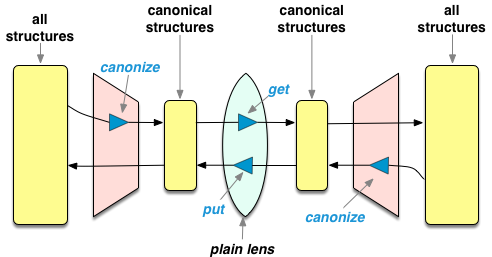
\includegraphics[width=0.7\textwidth]{canonizers-outside}
\caption{QRE Lens with ``Canonizers at the Edges''}
\label{fig:attheedges}
\end{figure}
Every QRE lens $q_1$ has a type $q_1: Q_1 \Leftrightarrow Q_2$ where $Q_1$ and $Q_2$
are QREs. In the get direction, a QRE lens $q_1: Q_1 \Leftrightarrow Q_2$ uses the
source QRE $Q_1$ to compute a unique representative for the data modulo the
equivalence relation defined by $Q_1$ and then applies the $\get$ function of a
bijective string lens $\ell_1$ to this representative. In the backward direction, $q_1$
operates similarly, but using the view QRE $Q_2$ and the $\lput$ function of
$\ell_1$.

Because the QREs $Q_1$ and $Q_2$ determine the internal formats for data after
canonization, and because the algorithm for synthesizing bijective string lenses is
directed by these formats, $Q_1$ and $Q_2$ are all that is required to
synthesize QRE lenses end-to-end. Indeed, we structured QRE lenses as bijective
lenses with canonizers at the edges, precisely to facilitate the use of this
synthesis algorithm.

On the other hand, our restriction that canonizers appear only at the edges
raises a key technical question:  Are we limiting the expressiveness of our
transformations by demanding all programs fit into this normal form?\bcp{I wish
we could have previewed this issue a bit more in the introduction, since it is
our main contribution.}  It turns out that we are not: any lens that uses
canonizers internally can be transformed into a lens that uses canonizers at
the edges. The main technical contribution of this paper is a proof of this
fact.

This technical investigation justifies replacing manually constructed lenses
using the QRE lens combinators with synthesized QRE lenses with canonizers at
the edges. For instance, after defining the \bibtex{} and EndNote QREs and
storing them in the variables \cd{bibtex} and \cd{endnote} respectively, then
all the code in Figure~\ref{fig:example-lens} may be replaced by a single call
to the synthesis prodedure:

\begin{lstlisting}
let bib_to_end : (lens in bibtex $\Leftrightarrow$ endnote) =
synth bibtex $\Leftrightarrow$ endnote using {(bib_example, end_example)}
\end{lstlisting}
\noindent Here, the generated  quotient lens synchronizes \cd{bibtex} and
\cd{endnote} formats, using \cd{bib_example} and \cd{end_example} (the two
concrete example strings given at the beginning of this section) to
disambiguate. In addition, and as we saw earlier with the definition of
\cd{c_to_s}, the synthesis procedure itself can be used to create lenses that
are in turn used to define other QREs.  The ability to intermix QRE
specification with QRE lens synthesis yields a powerful and flexible way of
creating bidirectional transformations.

\section{Quotient Regular Expressions}
A Quotient Regular Expression (or QRE) is a regular expression $R$ augmented
with syntax that expresses an equivalence relation on the language of $R$. This
section describes in further detail the set of QRE combinators that we described
in \cref{sec:example}.
\label{QRE}
\subsection{Syntax and Semantics of QREs}
Formally, the language of Quotient Regular Expressions (QREs) is given by the
following grammar:
\begin{align*}
Q := \; &R \sep \project{R}{s} \sep \squash{Q_1}{Q_2}{f} \sep
\perm{Q_1, \ldots, Q_n}{Q} \\
& | \; \normalize{R}{R'}{f} \sep Q_1 \semicolon Q_2 \sep Q_1 \cdot Q_2 \sep (Q_1
\sep Q_2) \sep Q^*,
\end{align*}
where $Q$ ranges over QREs, $R$ ranges over regular expressions, $f$ ranges over
functions between regular languages, and $s$ ranges over character strings.

Using the conventional notation that $\mathcal{L}(R)$ is the language accepted
by the regular expression $R$, then each QRE $Q$ enables us to express
\begin{enumerate}
  \item a regular expression $W(Q)$ (the ``whole'' of $Q$),
  \item an equivalence relation $\eqrel{Q}$ on $\mathcal{L}(W(Q))$,
  \item a regular expression $K(Q)$ (the ``kernel'' of $Q$)
  such that $\mathcal{L}(K(Q))$ forms a complete set of representatives for
  $\eqrel{Q}$, and
  \item a ``canonizing'' function\bcp{Why is it called ``canonizer'' rather
  than ``canonize''??}\sam{because \canonizer(Q) is a function}
  $\canonizer(Q):\mathcal{L}(W(Q)) \longrightarrow \mathcal{L}(K(Q))$ which
  given any $w \in \mathcal{L}(W(Q))$, computes $\canonizer(Q)(w)$ as the
  unique $k$ in $\mathcal{L}(K(Q))$ such that $k$ is equivalent to $w$ mod
  $\eqrel{Q}$
\end{enumerate}
Figures~\ref{fig:wk} gives the inductive definitions for the whole and
kernel languages $W(Q)$ and $K(Q)$ of a QRE.
\begin{figure}[t]
\centering
\[
\begin{array}{l@{\quad}l@{\quad}l}

Q & W(Q) & K(Q) \\ \hline
R & R & R \\
\project{R}{s} & R & s \\
\squash{Q}{Q_1}{f} & W(Q) \sep W(Q_1) & K(Q_1) \\
\normalize{R}{R'}{f} & R & R' \\
Q_1 \; ; \; Q_2 & W(Q_1) & K(Q_2) \\
Q_1 \cdot Q_2 & W(Q_1) \cdot W(Q_2) & K(Q_1) \cdot K(Q_2) \\
Q_1 \sep Q_2 & W(Q_1) \sep W(Q_2) & K(Q_1) \sep K(Q_2) \\
Q^* & W(Q)^* & K(Q)^* \\
\end{array}
\]
\[
\begin{array}{r@{\quad}l}
W( \perm{Q_1, \ldots, Q_n}{Q} ) = &
\bigcup \limits_{\sigma \in S_n} W(c_{\sigma(1)}) \cdot W(Q) \cdot \ldots \cdot
W(Q) \cdot W(c_{\sigma(n)})\\
K( \perm{Q_1, \ldots, Q_n}{Q} ) = & K(Q_1) \cdot K(Q) \cdot \ldots \cdot K(Q)
\cdot K(Q_n)
\end{array}
\]
\caption{Whole and Kernel Regular Expressions}
\label{fig:wk}
\end{figure}
The \textit{squash} and \textit{permutation} combinators give the two
interesting definitions. If $Q = \squash{Q_1}{Q_2}{f}$, then the whole language
of $Q$ is $W(Q_1) \sep W(Q_2)$. This is because the \textit{squash} combinator
takes the whole language $W(Q_1)$ of $Q_1$, the whole language $W(Q_2)$ of $Q_2$
and a function $f : \mathcal{L}(W(Q_1)) \longrightarrow \mathcal{L}(W(Q_2))$,
maps $\mathcal{L}(W(Q_1))$ into $\mathcal{L}(W(Q_2))$ using $f$ and then
canonizes $W(Q_2)$ into $K(Q_2)$ using $\canonizer(Q_2)$.

For the $\perm{Q_1, \ldots, Q_n}{Q}$ combinator, the whole language is the
union of languages of the form $W(c_{\sigma(1)}) \cdot W(Q) \cdot \ldots \cdot
W(Q) \cdot W(c_{\sigma(n)})$ for any permutation $\sigma$ in $S_n$, where
$S_n$ is the set of all permutations of the numbers $1$ to $n$. This is because
the \textit{permutation} combinator allows for the string to match any
permutation the $Q_i$'s while also taking into account the separator $Q$ in
between each of the $Q_i$'s. The kernel of the \textit{permutation} combinator
is the language $K(Q_1) \cdot K(Q) \cdot \ldots \cdot K(Q) \cdot K(Q_n)$,
because the canonical permutation is the identity permuation, with each of the
parts of the string that match $Q_i$ and $Q$ canonized into $K(Q_i)$ and $K(Q)$
respectively.

Figure~\ref{fig:canonizers} gives the inductive definitions of the
$\canonizer{}$ function for each QRE.
\begin{figure}[t]
\begin{center}
\[
\begin{array}{l@\quad l @\quad l}
\canonizer(R) &=& id_{\mathcal{L}(R)} \\
\canonizer(\project{R}{s})(w) &=& s\\
\canonizer(\squash{Q_1}{Q_2}{f})(w) &=&
\begin{cases}
\canonizer(Q_1)(f(w)) & \text{if } w \in \mathcal{L}(W(Q_1))\\
\canonizer(Q_2)(w) & \text{otherwise}
\end{cases}\\
\canonizer(\normalize{R}{R'}{f}) &=& f\\
\canonizer(Q_1 \; ; \; Q_2) &=& \canonizer(Q_2) \circ \canonizer(Q_1)\\
\canonizer(Q_1 \cdot Q_2) &=& \canonizer(Q_1) \cdot \canonizer(Q_2)\\
\canonizer(Q_1 \sep Q_2)(w) &=&
\begin{cases}
\canonizer(Q_1)(w) & \text{if } w \in \mathcal{L}(W(Q_1))\\
\canonizer(Q_2)(w) & \text{if } w \in \mathcal{L}(W(Q_2))\\
\end{cases}\\
\canonizer(Q^*) &=& \canonizer(Q)^* \\
\end{array}
\]
\end{center}
\begin{align*}
&\canonizer(\perm{Q_1, \ldots, Q_n}{Q})(r_{\sigma(1)}
\cdot s_1 \cdot \ldots \cdot s_{n-1} \cdot r_{\sigma(n)})\\
&= (\canonizer(Q_1)(r_1)) \cdot (\canonizer(Q)(s_1)) \cdot \ldots \cdot
(\canonizer(Q_n)(r_n))
\end{align*}
\caption{QRE canonizers}
\label{fig:canonizers}
\end{figure}
Again, the \textit{permutation} combinator gives the most interesting
definition,
\begin{align*}\canonizer(\perm{Q_1, \ldots, Q_n}{Q})(r_{\sigma(1)}
\cdot s_1 \cdot \ldots \cdot s_{n-1} \cdot r_{\sigma(n)}) \\
= (\canonizer(Q_1)(r_1)) \cdot (\canonizer(Q)(s_1)) \cdot \ldots \cdot
(\canonizer(Q_n)(r_n))
\end{align*}
\noindent which, as we have explained, is defined so that the strings that match
$Q_i, Q$ are placed in the canonical permutation which is the identity
permutation before $\canonizer(Q_i)$ and $\canonizer(Q)$ are applied
respectively.

Finally, Figure ~\ref{fig:relations} gives the inductive definition of the
equivalence relation $\eqrel{Q}$. This is the set-theoretic semantics of QREs
as an equivalence relation on a regular language.

\begin{figure}[t]
\centering
\[
\begin{array}{l@{}l@{\ \ }l}
w \; \equiv_R \; w' &\iff& w = w' \\
w \; \equiv_{\project{R}{s}} \; w' && \text{for all }w, w'\\
w \; \equiv_{\squash{Q_1}{Q_2}{f}} \; w' &\iff& f(w) \equiv_{Q_2} w'
\text{ or } w \equiv_{Q_2} w' \\
w \; \equiv_{\normalize{R}{R'}{f}} \; w' &\iff&
f(w)=f(w') \text{ or }w = w'\\
w \; \equiv_{Q_1 \; ; \; Q_2} \; w' &\iff& \exists k, k' \in
\mathcal{L}(K(Q_2)) \text{ such that } w \; \equiv_{Q_1} \; k, \; w' \;
\equiv_{Q_1} \; k', \text{ and } k \; \equiv_{Q_2} \; k'\\
w \; \equiv_{Q_1 \cdot Q_2} \; w'  &\iff& w = r_1
\cdot r_2, \; w' = {r'}_1 \cdot {r'}_2 \text{ with } r_1 \; \equiv_{Q_1}
\; {r'}_1, \; r_2 \; \equiv{Q_n} \; {r'}_2\\
w \; \equiv_{Q_1 \sep Q_2} \; w' &\iff& w \; \equiv_{Q_1} \; w'
\text{ or } \; w \; \equiv_{Q_2} \; w'\\
w \; \equiv_{Q^*} \; w' &\iff& w = r_1 \cdot \ldots \cdot r_n, \; w'
= {r'}_1 \cdot \ldots \cdot {r'}_n \text{ and } r_i \equiv_{Q} \; {r'}_i
\\
w \; \equiv_{\perm{Q_1, \ldots, Q_n}{Q}} \; w' &\iff& w = r_{\sigma(1)}
\cdot s_1 \cdot \ldots \cdot s_{n-1} \cdot r_{\sigma(n)}, \;
w' = {r'}_{\theta(1)} \cdot s'_1 \cdot \ldots \cdot s'_{n-1}
\cdot {r'}_{\theta(n)} \\
& & \text{for some } \sigma, \theta \in S_n, \text{ with } r_i \;
\equiv_{q_i} \; r'_i \text{ and } s_k \; \equiv_{Q} \; s'_{k}
\end{array}
\]
\caption{QRE Equivalence Relations}
\label{fig:relations}
\end{figure}
\subsection{Well Formed QREs}
\subsubsection{Completeness of {\em normalize}}
Before we present the full inference rules, for QREs, we discuss the {\em
normalize} QRE which is special in two main ways, the first of which has to do
with the premises in its inference rule:
\begin{prooftree}
\AxiomC{$\mathcal{L}(R') \subseteq \mathcal{L}(R)$}
\AxiomC{$f : \mathcal{L}(R) \longrightarrow \mathcal{L}(R')$}
\AxiomC{$f$ is surjective}
\AxiomC{$f = f^2$}
\RightLabel{(Normalize)}
\QuaternaryInfC{$\wf{\normalize{R}{R'}{f}}$}
\end{prooftree}
In order for the {\em normalize} QRE to be well-formed, then canonizing function
$f$ used by this combinator must be surjective and idempotent. Unfortunately,
verifying that a function satisfies these properties is in general undecidable.
Nonetheless, we allow a programmer to use normalize at their own risk without
checking these side conditions.

We do this firstly because the {\em normalize} combinator allows one to express
equivalence relations that are either difficult to define, or that cannot be
defined using the other combinators. Secondly, the {\em normalize} canonizer
enjoys the property that each of the other combinators $Q$ is semantically
equivalent to $\normalize{W(Q)}{K(Q)}{f}$ for some surjective, idempotent
function $f : \mathcal{L}(W(Q)) \longrightarrow \mathcal{L}(K(Q))$; this is the
second property that distinguishes the {\em normalize} combinator from the other
QREs. The {\em normalize} combinator hence gives a sufficient condition for
potential QREs to be ``well-behaved'', particularly with respect to the
strategy for synthesizing quotient lenses which we shall introduce in
Section~\ref{synth}. This is the
\subsubsection{Ambiguity}
Another issue which we address before presenting the full set of inference
rules for QREs, we discuss the issue of {\em ambiguity}, which appears in the
premises of the inference rules for the regular combinators. If $Q_1$ and $Q_2$
are QREs, then when applying the regular combinators to QREs, we require that
if a string $s$ matches any of the regular expressions $W(Q_1) \cdot W(Q_2)$,
\quad $W(Q_1) \sep W(Q_2)$, \quad $W(Q_1)^*$, \quad $K(Q_1) \cdot K(Q_2)$,
\quad $K(Q_1) \sep K(Q_2)$, \quad $K(Q_1)^*$, then $s$ matches that regular
expression in only one way.

Formally, we say that regular expressions $R$ and $S$ are
\textit{unambiguosly concatenable}, written $R \cdot^! S$ if for all strings
$r, r' \in \mathcal{L}(R)$ and $s, s' \in \mathcal{L}(S)$, if $r \cdot s = r'
\cdot s'$, then $r = r'$ and $s = s'$. We say that a regular expression $R$ is
\textit{unambiguosly iterable}, written $R^{*!}$ if for all strings $r_1,
\ldots, r_m$ and $r'_1, \ldots, r'_n \in \mathcal{L}(R)$, if $r_1 \cdot \ldots
\cdot r_m = r'_1 \cdot \ldots \cdot r'_n$, then $m = n$ and $r_i = r'_i$. We say
that a regular expression $R$ is \textit{strongly unambiguous}\cite{Sippu1988}
if and only if (1) $R = \varnothing$, or (2) $R = S_1 \cdot S_2$ with $S_1,
S_2$ strongly unambiguous and $S_1 \cdot^! S_n$, or (3) $R = S_1 \sep S_2$ with
$S_1, S_2$ strongly unambiguous and $\mathcal{L}(S_1) \cap \mathcal{L}(S_2) =
\varnothing$, or (4) $R = S^*$ with $S$ strongly unambiguous and $S^{*!}$.

Strong unambiguity is necessary in the premises of the regular QRE combinators
because it ensures that the canonizing function of a QRE is well-defined.
For example consider the QRE \lstinline{"a"* . (project "a"* $\to$ "a")}. The
behaviour of this QRE is not-well defined since the string
\cd{"aaa"} can be canonized to any of \cd{"a"}, \cd{"aa"}, or \cd{"aaa"}
depending on how \cd{"aaa"} is parsed. We also require that the regular
combinators applied to the kernels of QREs be unambiguous since the underlying
bijective string lens of a QRE lens operates on kernels, and bijective string lenses
impose the same unambiguity restrictions so that they too are well defined as
functions.

Figure~\ref{fig:qrerules} gives the inference rules for deriving well-formed
QREs.
\begin{figure}[tp!]
\begin{center}
\AxiomC{$R$ is strongly unambiguous}
\RightLabel{(Id)}
\UnaryInfC{$\wf{\mathit{id}(R)}$}
\DisplayProof
\hskip 1.5em
\AxiomC{$s \in \mathcal{L}(R)$}
\RightLabel{(Project)}
\UnaryInfC{$\wf{\project{R}{s}}$}
\DisplayProof
\hskip 1.5em
\end{center}

\begin{prooftree}
\AxiomC{$\wf{Q_i, Q}$}
\RightLabel{(Perm)}
\AxiomC{${\substack{\forall \sigma \neq \theta, \; W(c_{\sigma(1)}) \cdot W(Q)
\cdot \ldots \cdot W(c_{\sigma(n)})\\ \cap W(c_{\theta(1)}) \cdot W(Q)
\cdot \ldots \cdot W(c_{\theta(n)}) =\varnothing}}$}
\AxiomC{$K(Q_1) \cdot^! K(Q) \cdot^! \ldots \cdot^! K(Q) \cdot^! K(Q_n)$}
\TrinaryInfC{$\wf{\perm{Q_1, \ldots, Q_n}{Q}}$}
\end{prooftree}

\begin{center}
\AxiomC{$\wf{Q_1, Q_2}$}
\AxiomC{$\mathcal{L}(W(Q_1)) \cap \mathcal{L}(W(Q_2)) = \varnothing$}
\AxiomC{$f : \mathcal{L}(W(Q_1)) \longrightarrow \mathcal{L}(W(Q_2))$}
\RightLabel{(Squash)}
\TrinaryInfC{$\wf{\squash{Q_1}{Q_2}{f}}$}
\DisplayProof
\end{center}
\begin{center}

\begin{prooftree}
\AxiomC{$\mathcal{L}(R') \subseteq \mathcal{L}(R)$}
\AxiomC{$f : \mathcal{L}(R) \longrightarrow \mathcal{L}(R')$}
\AxiomC{$f$ is surjective}
\AxiomC{$f = f^2$}
\RightLabel{(Normalize)}
\QuaternaryInfC{$\wf{\normalize{R}{R'}{f}}$}
\end{prooftree}

\end{center}
\begin{center}
\AxiomC{$\wf{Q_1, Q_2}$}
\AxiomC{$K(Q_1) = W(Q_2)$}
\RightLabel{(Compose)}
\BinaryInfC{$\wf{Q_1 \; ; \; Q_2}$}
\DisplayProof
\hskip 1.5em
\AxiomC{$\wf{Q}$}
\AxiomC{$W(Q)^{*!}$}
\AxiomC{$K(Q)^{*!}$}
\RightLabel{(Star)}
\TrinaryInfC{$\wf{Q^*}$}
\DisplayProof
\end{center}
\begin{center}

\begin{center}
\AxiomC{$\wf{Q_1, Q_2}$}
\AxiomC{$W(Q_1) \cdot^! W(Q_2)$}
\AxiomC{$K(Q_1) \cdot^! K(Q_2)$}
\RightLabel{(Concat)}
\TrinaryInfC{$\wf{Q_1 \cdot Q_2}$}
\DisplayProof
\end{center}

\begin{center}
\AxiomC{$\wf{Q_1, Q_2}$}
\AxiomC{$W(Q_1) \cap W(Q_2) = \varnothing$}
\RightLabel{(Union)}
\BinaryInfC{$\wf{Q_1 \sep Q_2}$}
\DisplayProof
\
\end{center}
\end{center}
\caption{Well-formed QREs}
\label{fig:qrerules}
\end{figure}
As we already mentioned, the unambiguity conditions come into play when defining
QREs using the regular combinators. For example, the (Concat) inference rule
for concatenation says that the concatenation $Q_1 \cdot Q_2$ of QREs $Q_1$ and
$Q_2$ is well formed only if the concatentions of $W(Q_1)$ and $W(Q_2)$, and
$K(Q_1)$ and $K(Q_2)$ are unambiguous.

The most complicated inference rule is the (Perm) rule for the
\textit{permutation} combinator. The second hypothesis for the
\textit{permutation} rule says that for any two different permutations $\sigma$
and $\theta$, the languages $W(c_{\sigma(1)}) \cdot W(Q) \cdot \ldots \cdot
W(c_{\sigma(n)})$ and $W(c_{\theta(1)}) \cdot W(Q) \cdot \ldots \cdot
W(c_{\theta(n)})$ must be disjoint. This is because any string that matches the
\textit{permutation} combinator matches the language $W(c_{\theta(1)}) \cdot
W(Q) \cdot \ldots \cdot W(c_{\theta(n)})$ for some permutation $\theta$, so we
require that these regular expressions be disjoint.
%
The third hypothesis says that the regular expression $K(Q_1) \cdot K(Q)
\cdot \ldots \cdot K(Q) \cdot K(Q_n)$ must be unambiguous. This is because the
underlying lens that maps to or from a \textit{permutation} QRE operates on
the language $K(Q_1) \cdot K(Q) \cdot \ldots \cdot K(Q) \cdot K(Q_n)$ which is
the kernel of the \textit{permutation} QRE. As we mentioned, the underlying
lens will require that the source and target regular expressions of the lens be
unambiguous so that the lens can match strings uniquely.


\section{QRE Lenses}
\label{QRE-lenses}
As we have seen, QREs express a broad class of equivalence relations
directly on regular languages. QREs are therefore a good \textit{specification}
language for quotient lenses. In this section we introduce \textit{QRE Lenses},
a class of quotient lenses that map between data that is specified using QREs.

First we give the formal definition of a {\em bijective quotient lens}; QRE
lenses are a specific class of bijective quotient lenses that map between data
that is specified by QREs. Given regular expressions $R, S$ and equivalence
relations $\sim_R$ and $\sim_S$ defined on $\mathcal{L}(R)$ and $\mathcal{L}(S)$,
we define a {\em bijective quotient lens} $q : R /{\sim_R} \Leftrightarrow
S/{\sim_S}$ to be a pair of functions $q.\get :
\mathcal{L}(R) \longrightarrow \mathcal{L}(S)$ and $q.\lput : \mathcal{L}(S)
\longrightarrow \mathcal{L}(R)$ such that for all $r \in \mathcal{L}(R)$ and $s
\in \mathcal{L}(S)$, we have $q.\lput(q_1.\get(r)) \sim_R r$ and
$q.\get(q_1.\lput(s)) \sim_R s$. Moreover, if $r \sim_R r'$, then $q.\get(r) =
q.\get(r')$, and if $s \sim_S s'$, then $q.\lput(s) = q.\lput(s')$.

In words, a bijective quotient lens $q$ from $R$ to $S$ modulo $\sim_R$
and $\sim_S$ is a pair of functions $q.\get$ and $q.\lput$ such that
$q.\get$ respects $\sim_R$ and $q.\lput$ respects $\sim_S$, and such that
the {\em get} and {\em put} functions lifted to $\mathcal{L}(R)/{\sim_R}$ and
$\mathcal{L}(S)/{\sim_S}$ are mutual inverses.

These laws are similar to the laws for bijective lenses
\cref{bijectivelenslaws}, except that the  equality restrictions in the
bijective lens laws are loosened to allow for equivalence relations. Also, the
condition that $r \sim_R r'$ implies $q.\get(r) = q.\get(r')$ ensures that the
{\em get} function induced on the equivalence classes if $\equiv_c$ is
well-defined, and similarly for the {\em put} function. 

Having identified QREs as a natural way of specifing equivalence relations on
regular expressions, a natural next step in defining quotient lenses is to map
between two QREs via a bijection between their; this is our
approach in defining {\em QRE lenses}.

More concretely, in order to define a language of QRE lenses, our approach is
to (1) define a language of bijections (Section \ref{subsec:bijective-lenses}),
and then (2) add quotients by allowing canonizers to be prepended or postpended
to bijections and (3) allowing composition of such quotient lenses via the
regular operators and functional composition
(Sections \ref{subsec:qre-lenses-syntax} and \ref{subsec:qre-lenses-semantics}).

However, we also have a secondary objective, which is to support synthesis of
lenses: When provided with QREs describing the source and target languages, we
would like to be able to generate quotient lenses automatically. One way to do
that is to generate canonizers $\canonizer(Q_1)$ and $\canonizer(Q_2)$ from QREs
$Q_1$ and $Q_2$ and then to synthesize bijective lenses between the kernel
languages for $Q_1$ and $Q_2$.

Unfortunately, the composition of two such quotient lenses does not have have
the form of a bijective lens with canonizers at the edges. Hence, an important
technical question is whether we give up expressiveness if we restrict
ourselves to this form. Thankfully, this turns out not to be an issue if
the bijections that we use to define QRE lenses are derived using a particular
set of combinators that we describe in the next section.

\subsection{Bijective String Lenses}
\label{subsec:bijective-lenses}
We define the set of \textit{bijective string lenses} to be the set of
bijections between regular languages constructed using the following combinators.

$$\ell := \mathit{id} \; (R) \sep \const(s_1, s_2) \sep  \swap(\ell_1, \ell_2)
\sep \ell_1 \cdot \ell_2 \; |  \; (\ell_1 \sep \ell_2) \sep \ell^* \; | \;
\ell_1 \; ; \;  \ell_2,$$ where $R$ ranges over regular expressions and $s$
ranges over character strings.

The $\mathit{\const}(s, t)$ lens replaces the string $s$ with $t$ in the source
data in the forward direction, and $t$ with $s$ in the target data in the
backward direction, while $\mathit{id}(R)$ applies the identity function to the
source and target  in $\mathcal{L}(R)$ in both directions. The composition lens
$\ell_1 \; ; \; \ell_2$ applies $\ell_1$ followed by then $\ell_2$ to the
source in the forward direction, and applies $\ell_2$ followed by $\ell_1$ to
the target in the backward direction. The lens $\ell_1 \cdot \ell_2$ first
splits the string $s$ into $s_1$ and $s_2$, applies $\ell_1$ and $\ell_2$ to
$s_1$ and $s_2$ to get $t_1$ and $t_2$ respectively, then concatenates $t_1$
and $t_2$ and returns $t_1 \cdot t_2$ as the final result in the forward
direction. $\ell_1 \cdot \ell_2$ operates similarly in the backward direction,
but with $s, s_1$ and $s_2$ substituted for $t, t_1$ and $t_2$. The
$\mathit{\swap} \; (\ell_1, \ell_2)$ lens operates like $\ell_1 \cdot \ell_2$,
except that it swaps $t_1$ and $t_2$ before concatenating the two for a final
result of $t_2 \cdot t_1$ in the forward direction. In the backward direction,
$\mathit{\swap}(\ell_1, \ell_2)$ first undoes the \swap, then behaves like
$cdot$. The $\ell_1 \; | \; \ell_2$ lens chooses to apply $\ell_1$ or $\ell_2$
depending on whether the source (resp. target) data is matched by $\ell_1$ or
$\ell_2$ in the forward (resp. backward direction). The $\ell^*$ lens splits the
string $s$ into strings $s_1, \ldots, s_n$, applies $\ell_1$ to each $s_i$ to
get $t_i$, and then concatenates each of the $t_i$'s for a final result of $t_1
\cdot \ldots \cdot t_n$ in the forward direction. The iteration lens $\ell^*$
operates similarly in the backward direction, but with $s, s_i$ substituted for
$t, t_i$.

The denotation of a lens $\ell_1$ is $\llbracket \ell_1 \rrbracket \subseteq
\mathit{String} \times \mathit{String}$. If $(s_1, s_2) \in \llbracket \ell_1
\rrbracket$, then $\ell_1$ maps between $s_1$ and $s_2$.
\begin{align*}
\llbracket R \rrbracket &= \{(r, r) \sep r \in \mathcal{L}(R)\}\\
\llbracket \const(r, s) \rrbracket &= \{(r, s)\}\\
\llbracket \swap(\ell_1, \ell_2) \rrbracket &= \{(s \cdot t, t' \cdot s') \sep
(s, s') \in \llbracket \ell_1 \rrbracket \text{ and } (t, t') \in \llbracket
\ell_2 \rrbracket\}\\
\llbracket \ell_1 \cdot \ell_2 \rrbracket &= \{(s \cdot t, s' \cdot t) \sep
(s, s') \in \llbracket \ell_1 \rrbracket \text{ and } (t, t') \in \llbracket
\ell_2 \rrbracket\}\\
\llbracket \ell_1 \sep \ell_2 \rrbracket &= \{(s \cdot t) \sep
(s, t) \in \llbracket \ell_1 \rrbracket \text{ or } (s, t) \in \llbracket
\ell_2 \rrbracket\}\\
\llbracket \ell^* \rrbracket &= \{(s_1 \cdot \ldots \cdot s_n, t_1 \cdot \ldots
\cdot t_n) \sep (s_i, t_i) \in \llbracket \ell \rrbracket \text{ for } 1
\leq i \leq n\}\\
\llbracket \ell_1 \; ; \; \ell_2 \rrbracket &= \{(r, t) \sep \text{there exists }s
\text{ such that } (r, s) \in \llbracket \ell_1 \rrbracket \text{ and } (s, t)
\in \llbracket \ell_2 \rrbracket\}
\end{align*}

Each bijective string lens $\ell$ has a type $\ell : R \Leftrightarrow S$ where
$R$ and $S$ are regular expressions. If $\ell : R \Leftrightarrow S$, then the
source language of $\ell$ is $\mathcal{L}(R)$ and the target language of $\ell$
is $\mathcal{L}(S)$. IThe final rule in the figure deserves special attention.
It states that a lens $\ell : R \Leftrightarrow S$ can also be considered to be
of type $\ell : R' \Leftrightarrow S'$ provided that $R$ (resp. $S$) can be
proven to be equivalent to $R'$ (resp. $S$) from the star-semiring axioms
(associativity and commutativity of | and $\cdot$, identity of the empty string
$\epsilon$, distibutivity of $\cdot$ over |, annihilative property of
$\varnothing$ with respect to $\cdot$, and that $R^* = \epsilon \; | \; R \cdot
R* = \epsilon \; | \; R^* \cdot R$ for all $R$):

\begin{prooftree}
\AxiomC{$\ell_1 : R \Leftrightarrow S$}
\AxiomC{$R \equiv^s R'$}
\AxiomC{$S \equiv^s S'$}
\TrinaryInfC{$\ell_1 : R' \Leftrightarrow S'$}
\end{prooftree}

\noindent
This rule makes it significantly more difficult to synthesize a bijective lens
from its type.\sam{Should we explain why?}

\begin{figure}[t]
\begin{center}
\AxiomC{$s_1 \in \Sigma^*$}
\AxiomC{$s_2 \in \Sigma^*$}
\BinaryInfC{$\mathit{\const} \; (s_1, s_t): s_1 \Leftrightarrow s_2$}
\DisplayProof
\hskip 1.5em
\AxiomC{$R$ is strongly unambiguous}
\UnaryInfC{$\mathit{id} \; (R): R \Leftrightarrow R$}
\DisplayProof
\end{center}

\begin{center}
\AxiomC{$\substack{\ell_1 : R_1 \Leftrightarrow S_1 \\ \ell_2 : R_2
\Leftrightarrow S_2}$}
\AxiomC{$\substack{R_1 \cdot^! R_2 \\S_1 \cdot^! S_2 }$}
\BinaryInfC{$\ell_1 \cdot \ell_2: R_1 \cdot R_2 \Leftrightarrow S_1 \cdot
S_2$}
\DisplayProof
\hskip 1.5em
\AxiomC{$\substack{\ell_1 : R_1 \Leftrightarrow S_1 \\ \ell_2 : R_2
\Leftrightarrow S_2}$}
\AxiomC{$\substack{R_1 \cdot^! R_2 \\ S_2 \cdot^! S_1}$}
\BinaryInfC{$\mathit{\swap} \; (\ell_1, \ell_2): R_1 \cdot R_2
\Leftrightarrow S_2 \cdot S_1$}
\DisplayProof
\end{center}

\begin{center}
\AxiomC{$\ell_1 : R_1 \Leftrightarrow R_2$}
\AxiomC{$\ell_2 : R_2 \Leftrightarrow R_3$}
\BinaryInfC{$\ell_1 \; ; \; \ell_2: R_1 \Leftrightarrow R_3$}
\DisplayProof
\hskip 1.5em
\AxiomC{$\substack{\ell_1 : R_1 \Leftrightarrow S_1 \\ \ell_2 : R_2
\Leftrightarrow S_2}$}
\AxiomC{$\substack{\mathcal{L}(R_1) \cap \mathcal{L}(R_2) =
\varnothing \\ \mathcal{L}(S_1) \cap \mathcal{L}(S_2) = \varnothing}$}
\BinaryInfC{$\ell_1 \sep \ell_2: R_1 \sep R_2 \Leftrightarrow S_1 \sep S_2$}
\DisplayProof
\end{center}

\begin{center}
\AxiomC{$\ell : R \Leftrightarrow S$}
\AxiomC{$R^{*!}$}
\AxiomC{$S^{*!}$}
\TrinaryInfC{$\ell^*: R \Leftrightarrow S$}
\DisplayProof
\hskip 1.5em
\AxiomC{$\ell : R \Leftrightarrow S$}
\AxiomC{$R \equiv^s R'$}
\AxiomC{$S \equiv^s S'$}
\TrinaryInfC{$\ell : R' \Leftrightarrow S'$}
\DisplayProof
\end{center}
\caption{Bijective String Lens Typing Rules}
\label{fig:lensrules}
\end{figure}

\subsection{Syntax of QRE Lenses}
\label{subsec:qre-lenses-syntax}
Having given a brief overview of the class of bijective string lenses, we now
introduce the class of QRE lenses. The language of QRE lenses is given by following
grammar:
$$ q := \kw {id}(R) \sep  \kw{const}(r, s) \sep q_1 \cdot q_2 \sep
\kw{swap}(q_1, q_2) \sep (q_1 \sep q_2) \sep q^* \sep q_1 \; ; \; q_2 \sep
\kw{lquot}(q, \ell) \sep \kw{rquot}(\ell, q)$$ where $R$ ranges over
regular expressions and $\ell$ ranges over bijective lenses.

TThe QRE lens combinators are the same as the bijective string lens
combinators but with two extra combinators where quotienting actually
occurs: tthe $\kw{lquot}$ and $\kw{rquot}$ combinators. The $\kw{lquot}(Q, q)$
combinator takes a quotient lens $q$ and quotients the source data using $Q$,
assuming that the source data forms a complete set of representatives for the
equivalence relation $\eqrel{Q}$. The $\kw{lquot}(q, Q)$ combinator does the
same but on the target data.

For example, recall that in the \bibtex{} to EndNote transformation, we had the
QREs \cd{bibtex} and \cd{endnote} and the bijective lens \cd{bib_to_end}
that maps between 
\cd{bibtex} and \cd{endnote}. The quotient lens that maps between
\cd{bibtex} and \cd{endnote} is then given by the following QRE lens:

\begin{lstlisting}
let bib_to_end_q : (lens in bibtex $\Leftrightarrow$ endnote) =  rquot (lquot(bibtex, bib_to_end), endnote)
\end{lstlisting}

\subsection{Semantics of QRE Lenses}
\label{subsec:qre-lenses-semantics}
Each QRE lens $q$ has a type $q : Q_1 \Leftrightarrow Q_2$ where $Q_1, Q_2$ are
QREs. If $q : Q_1 \Leftrightarrow Q_2$, then the source format is described by
$W(Q_1)$ and the canonical set of representative for the source data is
described by $K(Q_1)$.
Similarly, the target format is described by $W(Q_2)$ and the canonical set of
representatives for the target data is described by $K(Q_2)$. The underlying
lens of $q$ is a bijective lens $\ell : K(Q_1) \Leftrightarrow K(Q_2)$.

The denotation $\llbracket q \rrbracket$ of a QRE lens $q : Q_1 \Leftrightarrow
Q_2$ is a quotient lens $\llbracket q \rrbracket : W(Q_1)/{\eqrel{Q_1}}
\Longleftrightarrow W(Q_2)/{\eqrel{Q_2}}$. The typing rules and denotation of
QRE lenses are given in Figure~\ref{fig:qlenssemantics}.
\begin{figure}[ht]
TODO: Need to add some inferrence rules here.
\centering
\[
\begin{array}[b]{l@{\qquad}l}
\RuleSide{\ell : R \Leftrightarrow S}{\kw{lift}(\ell): id(R) \Leftrightarrow
id(S)}{\mathit{(Lift)}} &
\begin{array}[b]{rcl}
\llbracket \kw{lift}(\ell) \rrbracket.\get &=&  \llbracket \ell \rrbracket\\
\llbracket \kw{lift}(\ell) \rrbracket.\lput &=& \llbracket \ell \rrbracket^{-1}
\end{array}
\end{array}
\]
\[
\begin{array}[b]{c@{\qquad}c}
\RuleSide{q : Q_2  \Leftrightarrow Q_3 &
\wf{Q_1} &
K(Q_1) = W(Q_2)}
{\kw{lquot}(Q_1, q): Q_1 \; ; \; Q_2 \Leftrightarrow Q_3}{\mathit(Lquot)} &
\begin{array}[b]{rcl}
\llbracket \kw{lquot}(Q_1, q) \rrbracket.\get  &=& \llbracket q
\rrbracket.\get \circ \canonizer(Q_1)\\
\llbracket \kw{lquot}(Q_1, q) \rrbracket.\lput &=& \llbracket q
\rrbracket.\lput
\end{array}
\end{array}
\]

\[
\begin{array}[b]{c@{\qquad}c}
\RuleSide{q : Q_1 \Leftrightarrow Q_3 & \wf{Q_3} & W(Q_3) = K(Q_2)}
{\kw{rquot}(q, Q_1):Q_1 \Leftrightarrow Q_2 \; ; \; Q_3}{\mathit{(Rquot)}} &
\begin{array}[b]{rcl}
\llbracket \kw{rquot}(q, Q_1) \rrbracket.\get  &=& \llbracket q
\rrbracket.\get\\
\llbracket \kw{rquot}(q, Q_1) \rrbracket.\lput &=& \llbracket q
\rrbracket.\lput \circ \canonizer(Q_3)
\end{array}
\end{array}
\]

\[
\begin{array}[b]{l@{\qquad}c}
\RuleSide{q : Q_1 \Leftrightarrow Q_2 &
W(Q_1)^{*!},W(Q_2)^{*!} & K(Q_1)^{*!}, K(Q_2)^{*!}}
{{q}^* : {Q_1}^* \Leftrightarrow {Q_2}^*}{\mathit{(Star)}} &
\begin{array}[b]{rcl}
\llbracket {q}^* \rrbracket.\get  &=& (\llbracket q \rrbracket.\get)^*\\
\llbracket {q}^* \rrbracket.\lput &=& (\llbracket q \rrbracket.\get)^*
\end{array}
\end{array}
\]

\[
\begin{array}[b]{l@{\qquad}c}
\RuleSide{\substack{q_1 : Q_1 \Leftrightarrow d_1 \\ q_2 : Q_2 \Leftrightarrow
d_2} & {\substack{W(Q_1) \cdot^! W(Q_2)\\ K(Q_1) \cdot^! K(Q_2)}}
& {\substack{W(d_1) \cdot^! W(d_2)\\ K(d_1) \cdot^! K(d_2)}}}
{q_1 \cdot q_2: Q_1 \cdot Q_2 \Leftrightarrow d_1 \cdot d_2}{\mathit{(Concat)}}
&
\begin{array}[b]{rcl}
\llbracket q_1 \cdot q_2 \rrbracket.\get  &=& \llbracket q_1 \rrbracket.\get
\cdot \llbracket q_2 \rrbracket.\get\\
\llbracket q_1 \cdot q_2\rrbracket.\lput &=& \llbracket q_1 \rrbracket.\lput
\cdot \llbracket q_2 \rrbracket.\lput
\end{array}
\end{array}
\]

\[
\begin{array}[b]{l@{\qquad}c}
\RuleSide{\substack{q_1 : Q_1 \Leftrightarrow d_1 \\ q_2 : Q_2 \Leftrightarrow
d_2} & \substack{\mathcal{L}(W(Q_1)) \cap \mathcal{L}(W(Q_2)) = \varnothing
\\ \mathcal{L}(W(d_1)) \cap \mathcal{L}(W(d_2)) = \varnothing }}
{q_1 \sep q_2: (Q_1 \sep Q_2)\Leftrightarrow (d_1 \sep d_2)}{\mathit{(Or)}} &
\begin{array}[b]{rcl}
\llbracket q_1 \sep q_2 \rrbracket.\get(s) =
\begin{cases}
\llbracket q_1 \rrbracket.\get (s) & \text{if } s \in \mathcal{L}(W(Q_1))\\
\llbracket q_2 \rrbracket.\get (s) & \text{if } s \in \mathcal{L}(W(Q_2))\\
\end{cases}\\
\llbracket q_1 \sep q_2 \rrbracket.\lput(s) =
\begin{cases}
\llbracket q_1 \rrbracket.\lput (s) & \text{if } s \in \mathcal{L}(W(d_1))\\
\llbracket q_2 \rrbracket.\lput (s) & \text{if } s \in \mathcal{L}(W(d_2))\\
\end{cases}
\end{array}
\end{array}
\]

\begin{prooftree}
\AxiomC{$\substack{q_1 : Q_1 \Leftrightarrow Q_2 \\ q_2 : Q_3 \Leftrightarrow
Q_4}$}
\RightLabel{(Compose)}
\AxiomC{$\substack{\mathcal{L}(W(Q_2))= \mathcal{L}(W(Q_3)) \\ K(Q_2) \equiv^s
K(Q_3)}$}
\AxiomC{$\canonizer(Q_2) = \canonizer(Q_3)$}
\TrinaryInfC{$q_1 \; ; \; q_2: Q_1 \Leftrightarrow Q_4$}
\end{prooftree}
\begin{align*}
\llbracket q_1 \; ; \; q_2 \rrbracket.\get &= \llbracket q_2
\rrbracket.\get\circ \llbracket q_1 \rrbracket.\get\\
\llbracket q_1 \; ; \; q_2 \rrbracket.\lput &= \llbracket q_1 \rrbracket.\lput
\circ \llbracket q_2 \rrbracket.\lput
\end{align*}
\caption{Denotation and Typing Rules for QRE Lenses}
\label{fig:qlenssemantics}
\end{figure}
The trickiest typing rule is the typing rule for composition:

\begin{prooftree}
\AxiomC{$\substack{q_1 : Q_1 \Leftrightarrow Q_2 \\ q_2 : Q_3 \Leftrightarrow
Q_4}$}
\AxiomC{$\substack{\mathcal{L}(W(Q_2))= \mathcal{L}(W(Q_3)) \\ K(Q_2) \equiv^s
K(Q_3)}$}
\AxiomC{$\canonizer(Q_2) = \canonizer(Q_3)$}
\TrinaryInfC{$q_1 \; ; \; q_2: Q_1 \Leftrightarrow Q_4$}
\end{prooftree}

This derivation rule essentially says that the composition $q_1 \; ; \; q_2$ is
well defined if and only if the intermediary QREs $Q_3$ and $Q_4$ define the
same equivalence relation on regular languages that are equivalent modulo the
star-semiring axioms. The condition $\mathcal{L}(W(Q_2)) = \mathcal{L}(W(Q_3))$
says that the intermediary language is the same on both sides, while the
condition $K(Q_2) \equiv^s K(Q_3)$ says that the kernel regular expressions are
equivalent modulo the star-semiring axioms. Finally, the condition
$\canonizer(Q_2) = \canonizer(Q_3)$ says that $Q_2$ and $Q_3$ define the same
equivalence relation on $\mathcal{L}(W(Q_2))= \mathcal{L}(W(Q_3))$.

The semantics defined on QRE lenses imply the following theorem:
\begin{theorem}
If there is a derivation $q : Q_1 \Leftrightarrow Q_2$, then $\llbracket q
\rrbracket : W(Q_1)/{\eqrel{Q_1}} \Leftrightarrow W(Q_2)/{\eqrel{Q_2}}$ is a
well-defined quotient lens.
\end{theorem}
\subsection{Normal Forms of QRE Lenses}
Recall that our approach in defining QRE lenses is to have each QRE lens $q: Q_1
\Leftrightarrow Q_2$ be such that
\begin{align*}
\llbracket q \rrbracket.\get &= \ell \circ \canonizer(Q_1)\\
\llbracket q \rrbracket.\lput &= \ell^{-1} \circ \canonizer(Q_2)
\end{align*}
for some bijective lens $\ell$. In other words, each QRE lens is the same as a
bijective lens with canonizers at the edges. The following theorem,
which is the main technical contribution of this paper, confirms that this
indeed is the case:

\begin{theorem}\label{normal form}
If there is a derivation $q : Q_1 \Leftrightarrow Q_2$, then there exists a
bijective lens $\ell : K(Q_1) \Leftrightarrow K(Q_2)$ such that:
\begin{align*}
\llbracket q \rrbracket.\get &= \llbracket \ell \rrbracket\circ
\canonizer(Q_1)\\
\llbracket q \rrbracket.\lput &= \llbracket \ell \rrbracket^{-1} \circ
\canonizer(Q_2)
\end{align*}
\end{theorem}
\begin{proof}
The proof follows by induction on the derivation of $q : c \Leftrightarrow c$.
The most interesting part of the proof is the case for functional composition
as we must demonstrate that it is possible to eliminate the canonizers in the
middle of the term.

The derivation rule and denotation for composition are as follows:
\begin{prooftree}
\AxiomC{$\substack{q_1 : Q_1 \Leftrightarrow Q_2 \\ q_2 : Q_3 \Leftrightarrow
Q_4}$}
\AxiomC{$\substack{\mathcal{L}(W(Q_2))= \mathcal{L}(W(Q_3)) \\ K(Q_2) \equiv
K(Q_3)}$}
\AxiomC{$\canonizer(Q_2) = \canonizer(Q_3)$}
\TrinaryInfC{$q_1 \; ; \; q_2: Q_1 \Leftrightarrow Q_4$}
\end{prooftree}

\begin{align*}
\llbracket q_1 \; ; \; q_2 \rrbracket.\get &= \llbracket q_2 \rrbracket.\get\circ
\llbracket q_1 \rrbracket.\get\\
\llbracket q_1 \; ; \; q_2 \rrbracket.\lput &= \llbracket q_1 \rrbracket.\lput
\circ \llbracket q_2 \rrbracket.\lput
\end{align*}

By the induction hypothesis, there exist bijective lenses
$\ell_1 : K(Q_1) \Leftrightarrow K(Q_2)$ and $\ell_2 : K(Q_3) \Leftrightarrow
K(Q_4)$ such that
\begin{center}

\begin{tabular}{l l}
$\llbracket q_1 \rrbracket.\get = \llbracket \ell_1 \rrbracket \circ
\canonizer(Q_1)$ & $\llbracket q_2 \rrbracket.\get = \llbracket \ell_2
\rrbracket \circ \canonizer(Q_3)$ \\
$\llbracket q_1 \rrbracket.\lput = {\llbracket \ell_1 \rrbracket}^{-1} \circ
\canonizer(Q_2)$ & $\llbracket q_2 \rrbracket.\lput = {\llbracket \ell_2
\rrbracket}^{-1} \circ \canonizer(Q_4)$
\end{tabular}

\end{center}
%
Consequently,
\begin{align*}
\llbracket q_2 \rrbracket.\get \circ \llbracket q_1 \rrbracket.\get &=
(\llbracket \ell_2 \rrbracket \circ \canonizer(Q_3)) \circ (\llbracket \ell_1
\rrbracket \circ \canonizer(Q_1))\\
&= \llbracket \ell_2 \rrbracket \circ (\canonizer(Q_3) \circ \llbracket \ell_1
\rrbracket) \circ \canonizer(Q_1)\\
&= (\llbracket \ell_2 \rrbracket \circ \llbracket \ell_1 \rrbracket) \circ
\canonizer(Q_1)\\
&= \llbracket \ell_1 \; ; \; \ell_2 \rrbracket \circ \canonizer(Q_1)
\end{align*}
We are permitted to claim the third step from the second since
$\canonizer(Q_3)$ is the identity function on $K(Q_2)$ which is
syntactically equal to $K(Q_3)$ by assumption. A similar argument shows that
$$\llbracket q_1 \rrbracket.\lput \circ \llbracket q_2 \rrbracket.\lput =
\llbracket \ell_1 \; ; \; \ell_2 \rrbracket^{-1} \circ
\canonizer(Q_4)$$

The other cases of the proof are similar, proceeding by a
straightforward application of the induction hypothesis followed by unrolling
the equations that give the denotation for QRE lenses.  Full details can be
found in the appendix.
\end{proof}

\section{Synthesizing QRE Lenses}
\label{synth}

QRE lenses address some of the limitations of bijective lenses because a single
lens program expresses both the canonizers and the transformation between kernel
languages simultaneously, which reduces programmer effort.  But we can go even
further by recognizing that the type structure of QRE lenses contains
information that can be exploited to automatically synthesize lenses from their
types.  Rather than writing the QRE lens manually, the programmer can instead
specify the desired behavior of a lens by giving its interface types and providing
examples, if necessary, to disambiguate among possible implementations.  This
way of constructing lenses can often be much simpler than building them by
hand, as we saw in Section~\ref{sec:examplesynth}.

The Optician framework~\cite{optician} showed how to do such lens synthesis in
the case for bijective lenses. Here we show how to reduce QRE lens synthesis to
that case, so that we can re-use the Optician algorithm but in the more
expressive context of QRE lenses.  The basic idea is straightforward: we run the
Optician algorithm to synthesize a lens between the kernels of two QREs and then
apply the canonizers at the edges to recover a lens between the whole
languages.  This simple strategy turns out to be remarkably effective, and the
idea of using Optician in this way is part of the impetus\bcp{What was the
  other part??} for the design of our QRE lenses.  

The Optician synthesis algorithm works as follows. Given regular expressions $R$
and $S$ and a set of example input--output pairs
$\{(r_1, s_1),\allowbreak \ldots,\allowbreak (r_n, s_n)\}$, Optician will try to
find a bijective lens $\ell : R \Leftrightarrow S$ that that agrees on the
examples, \textit{i.e.}, it maps $r_i$ to $s_i$ in the forward direction and
$s_i$ to $r_i$ in the backward direction.  The Optician algorithm is guaranteed
to succeed (eventually!) if such a lens exists.    \saz{We should probably
  mention what happens if the examples aren't sufficient to uniquely
  determine the lens.}

In our setting, we want to synthesize a quotient lens $q: Q_1 \Leftrightarrow
Q_2$ from the QREs $Q_1$ and $Q_2$ and a set of example input-output pairs
$\{(x_1, y_1),\allowbreak \ldots,\allowbreak (x_n, y_n)\}$ where the $x_i$'s are
in $W(Q_1)$ and the $y_i$'s are in $W(Q_2)$. We furthermore wish $q$ to map the
equivalence class of $x_i$ to the equivalence class of $y_i$ and vice versa:
\begin{align*}
q.\get(x_i) &\equiv_{Q_2} y_i \text{, and}\\
q.\lput(y_i) &\equiv_{Q_1} x_i
\end{align*}
Our approach to synthesizing QRE lenses is guided by Theorem~\ref{normal form},
which says that, if there is a derivation $q : Q_1 \Leftrightarrow Q_2$ of a
QRE lens, then there exists a bijective lens $\ell : K(Q_1) \Leftrightarrow
K(Q_2)$ such that
\begin{align*}
\llbracket q \rrbracket.\get &= \llbracket \ell \rrbracket\circ \canonizer(Q_1)\\
\llbracket q \rrbracket.\lput &= \llbracket \ell \rrbracket^{-1} \circ
\canonizer(Q_2).
\end{align*}
\bcp{This math display and the previous one are punctuated perfectly: In the
first, the colon replaces a period at the end of the sentence (so no need
for another period at the end of the display).  In the second, the display
is punctuated as if it were inline.  Please go through and make sure all the
other displayed material follows one or the other of these rules.}

For the\bcp{why ``the''?  Are we talking about some set of QRE examples
  already?} QRE examples, the $x_i$'s are in $W(Q_1)$ and the $y_i$'s are 
in $W(Q_2)$, so we can construct ${x'_i} = \canonizer(Q_1)(x_i)$ in $K(Q_1)$
and ${y'_i} = \canonizer(Q_2)(y_i)$ is in $K(Q_2)$. To synthesize the
desired quotient lens $q: Q_1 \Leftrightarrow Q_2$ that is consistent with the
input-output examples $\{(x_1, y_1), \ldots, (x_n, y_n)\}$ it suffices to
synthesize a bijective lens $\ell : K(Q_1) \Leftrightarrow K(Q_2)$ that is
consistent with the canonized examples $\{({x'_1}, {y'_1}), \ldots, ({x'_n},
{y'_n})\}$ and then apply the canonizers at the outside. Our procedure for QRE
lens synthesis is thus
\begin{enumerate}
  \item
  Compute $K(Q_1)$, $K(Q_2)$,
  \item
  Compute $\{({x'_1}, {y'_1}), \ldots, ({x'_n}, {y'_n})\}$ where ${x'_i} =
  \canonizer(Q_1)(x_i)$ and ${y'_i} = \canonizer(Q_2)(y_i)$,
\item Synthesize, using Optician's algorithm, a bijective lens
  $\ell : K(Q_1) \Leftrightarrow K(Q_2)$ that is consistent with the examples
  $\{({x'_1}, {y'_1}),\allowbreak \ldots,\allowbreak ({x'_n}, {y'_n})\}$
  \item
  Return $q = \kw{rquot}(\kw{lquot}(Q_1, \ell), Q_2) : Q_1 \Leftrightarrow
  Q_2$ \bcp{punctuate this enumeration as if it were running text: ``, and''
  at the end of (3) and period here.  And lowercase letters at the
  beginnings of the items.}
\end{enumerate}

\saz{Do we want to state formally the completeness of this algorithm?}\BCP{+1}

Returning to the \bibtex{} to EndNote transformation of
Section~\ref{sec:examplesynth}, we had the QREs \cd{bibtex} and \cd{endnote}
describing a \bibtex{} record and an Endnote record respectively. We also had
the example pair \cd{(bib_example , end_example)} where

\begin{center}
\begin{minipage}{2.5in}
\begin{lstlisting}
bib_example =
"@Book {Lovelace,
 Author = \"Ada Lovelace\",
 Title = {Generic Title},
}"
\end{lstlisting}
\end{minipage}
\begin{minipage}{1.5in}
\begin{lstlisting}
end_example =
"%0 Book
 %T Generic Title
 %A Ada Lovelace
 %F Lovelace"
\end{lstlisting}
\end{minipage}
\end{center}

Since the transformation between the kernel of \cd{bibtex} and the kernel of
\cd{endnote} that maps \cd{bib_example} to \cd{end_example} can be
expressed as a bijective lens, we can synthesize a lens that maps between the
QREs \cd{bibtex} and \cd{endnote}, using the code below:

\begin{lstlisting}
let bib_to_end : (lens in bibtex <=> endnote) = 
  synth bibtex <=> endnote
  using {(bib_example, end_example)}
\end{lstlisting}

In this case, one example is sufficient to uniquely determine the desired
transformation.\SAZ{Is that true?}\BCP{Seems more likely that the desired
  transformation happened to be the first one that the synthesis algorithm
  reached.  Indeed, my intuition is that {\em every} synthesis problem with
  a finite set of examples has infinitely many solutions.  Is that right?}

\SAZ{We might want to say something more precise about the running time or
  expected performance of this algorithm, perhaps to set up the evaluation
  section.  Something along the lines of: ``Although the algorithm is complete
  in theory, in the worst case, it may take an unbounded [???IS THIS
  CORRECT?]\bcp{Surely it's bounded by some exponential formula involving the
    size of the inputs...?} 
  amount time to search for a satisfactory lens.  Nevertheless, this algorithm
  performs well in practice on numerous examples, as we show in the next
  section.} 

\section{Implementation and Evaluation}
\label{impl}

We have implemented QREs and the quotient lens synthesis algorithm described
above as an extension to the Boomerang
interpreter~\cite{boomerang,quotientlenses}. We have added QREs and QRE lens
synthesis tasks to Boomerang. Furthermore, these synthesis tasks evaluate to
Boomerang lens values, so Boomerang treats synthesized lenses the same as
hand-written ones. Intuition suggests that the increased expressiveness
of QREs should make many lens programming tasks easier, but we would like more
quantitative understanding of that claim. We thus conducted several experiments
that aim to provide answers to the following questions:

\begin{enumerate}
  \item Does synthesizing QRE lenses from QREs permit an easier development
  process than manually writing canonizers, and synthesizing the lenses between
  their canonized forms?  Does synthesizing QRE lenses from QREs permit an
  easier development process than writing the lenses by hand?
  
  \item Does the increase in expressivity gained from synthesizing from QREs
  permit synthesis of more useful lenses than existing approaches.  \bcp{Is
    this really an interesting empirical question?  Seems obvious, from the
    arguments we made in Section 2 and the intro.}\afm{I'm happy to remove it}
  
  \item Does our tool synthesize lenses fast enough to be used as part of a
  standard development process?
\end{enumerate}

All evaluations were performed on a 2.5 GHz Intel Core i7 processor with 16 GB
of 1600 MHz DDR3 running macOS High Sierra.


\subsection{Benchmark Suite Construction}

To evaluate our QRE implementation, we constructed a set of lens synthesis tasks
drawn from two sources:
\begin{enumerate}
\item 39 of our benchmarks were adapted from the evaluation of the original
  Optician system.  These benchmarks are a combination of custom benchmarks,
  benchmarks derived from FlashFill~\cite{flashfill}, and benchmarks
  derived from Augeas~\cite{augeas2}. In the pre-QRE version of
  Optician, many of these data formats had to be modified to work with the
  bijectivity constraints that Optician required.  For instance, when one format
  permits whitespace where the other does not allow it, the original versions of
  benchmark formats were modified to allow more whitespace, thereby restoring
  bijectivity.  With the new QRE support, we were able to remove these
  alterations when porting these benchmarks.  (This experience alone suggests
  that QREs make the lens development process easier.)
  
\item The remaining eight benchmarks were derived from datasets found at 
  data.gov. These datasets include census
  population data, wage comparison data, demographics statistics data and
  crime index data. We chose these datasets since they were stored in XML, CSV
  and RDF formats which are more easily specified using regular expressions than
  plain text or PDF documents.  \BCP{Besides differing formats, why did we
    include these eight new 
    ones?  Are they significantly different (more complex, exercising
    different features of the synthesis algorithm or QRE syntax,
    ...)?}\afm{Solomon, could you fill this out?}
    \sam{Well these data formats were the ones I was playing with before we got
    the Augeus and flashfill examples. I chose them simply because they had
    formats which could be expressed using regular expressions. They basically
    use the same QREs as the flashfill and augeus examples, mostly the project
    QRE. The fields in these files are occur in the same order in each record;
    we tried using the perm combinator anyways but the synthesis algorithm took
    too long. I do not think that they are significantly different from the
    flashfill and augues examples.}
\end{enumerate}

\subsection{Easing the Development Process}

\begin{figure}[t]
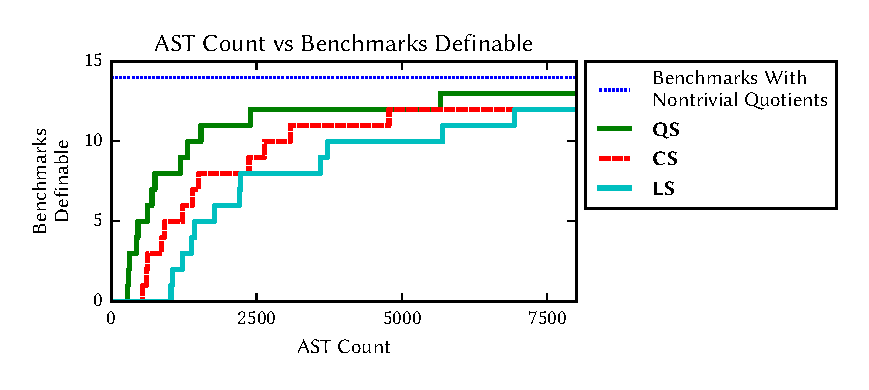
\includegraphics{generated-graphs/asts.eps}
\caption{Count of benchmark programs definable using a given AST count. We find
that it takes far fewer AST nodes to define benchmark lenses using QRE
synthesis than with Optician without QRE synthesis or without synthesis.}
\label{fig:asts}
\end{figure}

To get a sense of how much the new expressiveness that combining QRE lenses with
synthesis saves in terms of programmer effort, we compared the amount of code
that would need to be written for each of the lens benchmarks. We use number of
nodes in the abstract syntax tree as a measure of code size, and calculated
three quantities for each lens synthesis benchmark task. We only compared the
sizes on benchmarks where the canonization functions are nontrivial.
%
\begin{itemize}
  \item[\QRESize{}] the number of AST nodes in the QRE
  specifications (including examples)\saz{CHECK THIS}\afm{no but i'll add it in}
  \item[\CanonizerAndSpecSize{}]  the number of
  AST nodes in $W(q_1)$ summed with the number of AST nodes in $\canonizer(q_1)$
  \item[\LensAndSpecSize{}] the number of AST nodes
  in $W(q_1)$ summed with the number of AST nodes in the synthesized QRE lens.
\end{itemize}

The value of \QRESize{} is our measure of the programmer burden for
writing our benchmarks---it measures the number of AST nodes the programmer has
to write using the full expressiveness of QREs and synthesis.

The value of \CanonizerAndSpecSize{} estimates the burden for writing our
benchmarks within the Optician system, without QREs but still using
synthesis. (This is only an approximation, as both $W(q_1)$ and $\canonizer(q_1)$ are
automatically generated from the QRE, and it is possible that a human-written
version might be smaller.)

The value of \LensAndSpecSize{} estimates the burden in writing our benchmarks
in Boomerang, using neither QREs nor synthesis. (This is also an
approximation, as $W(q_1)$ and $\canonizer(q_1)$ and the bijective lens are all
automatically generated.)

Figure~\ref{fig:asts} shows the number of benchmarks that can be expressed using
at most a given number of AST nodes. For a given benchmark, we found \QRESize{}
to be about half as large as \CanonizerAndSpecSize, and about a third as large
as \LensAndSpecSize{}.\BCP{These are really the critical conclusions, and
  they are hard to see, the way the graph is drawn.  I wonder whether we
  could instead present with the individual examples on the X axis (sorted
  by number of AST nodes), with a bar above each one containing three
  regions, colored differently, for LS, CS-LS, and QC-CS...}\afm{will do} This suggests
that introducing QREs saves programmers 
significant effort compared to both Optician and basic Boomerang.

\subsection{Increasing Expressivity}

The pre-QRE version of Optician was only able to synthesize fully bijective data
transformations. Synthesizing from QREs loosens that restriction, making it
possible to synthesize data transformations involving bijections with
canonization functions. Because Optician could previously only synthesize
bijective lenses, some of the data formats in the example suite were modified to
include additional fields containing information should should be canonized from
the other format. In total, 12 of Optician's original benchmarks and 3 of the
data.gov benchmarks would require such additional fields when input to Optician
without QREs.

\subsection{Maintaining Competitive Performance}

\begin{figure}[t]
\centering
\begin{subfigure}[b]{.49\textwidth}
\centering
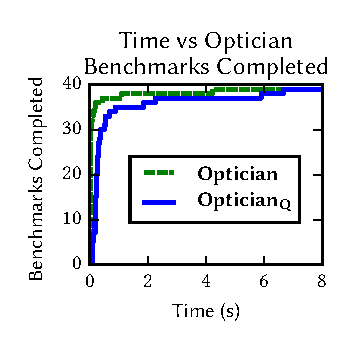
\includegraphics{generated-graphs/times_opt}
\caption{}
\label{subfig:lenssize}
\end{subfigure}
\begin{subfigure}[b]{.49\textwidth}
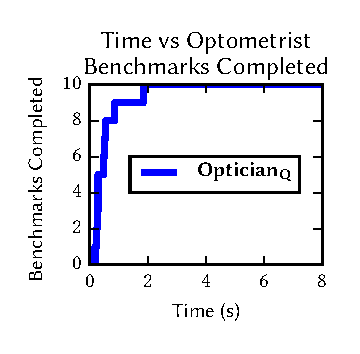
\includegraphics{generated-graphs/times_new.eps}
\caption{}
\label{subfig:examplesused}
\end{subfigure}
\caption{Runtimes of Optician and our system. In (a), we run Optician and our
  system on Optician's benchmarks. We find that there is only a negligible
  performance overhead incurred by using QREs. In (b), we run Optician with QREs
  on its benchmark suite. We find that it is able to synthesize all quotient
  lenses in under 20 seconds, and typically finished in under 5 seconds.
  \bcp{The left-hand graph, especially, is hard to make anything out of, because
    the curves are squished against the axes and have almost identical shapes.
    }\afm{will fix}}
\label{fig:times}
\end{figure}

To assess the performance impact of adding QRE support to Optician, we measured
the running time of the following configurations:
\begin{itemize}
  \item[\OpticianRuntime{}] pre-QRE Optician running on its own benchmarks.
  \item[\SystemOnOptician{}] Optician with QREs running on the pre-QRE benchmarks.
  \item[\SystemOnBenchmarks{}] Optician with QREs running on its own
  benchmarks. \BCP{What is the difference between QO and QQ??  The eight
    additional benchmarks?  Why not measure just these?  Seems like this
    graphj repeats some information from the one to the left, obscuring the
    new information.}\afm{will do}
\end{itemize}

We summarize the results of these experiments in Figure~\ref{fig:times}.  The
new version of Optician was able to synthesize all of pre-QRE Optician's
benchmarks at a speed competitive with the old version.  There is a small amount
of additional overhead introduced by QREs when calculating $W(q_1)$ and $K(q_1)$,
resulting in a very slight decrease in performance.

Also notable is one of the data.gov examples, which converts demographic
statistics by zip code from xml form into rdf form. Synthesizing this
transformation certainly took the longest, nearly fifteen seconds, where the
next slowest took hardly over five. To validate this performance was not due to
our overhead, we modified these format to be bijective, so the synthesis task
could be input into Optician. Optician took over 15 seconds synthesize this
modified lens. We believe this conversion took longer because the input formats
were exceptionally large, requiring conversions between over 40 fields, not due
to an overhead from synthesizing from QREs.
\section{Related Work}
\label{relwork}

\iffalse
Bidirectional transformations have been used in diverse areas of computing
where they arise as parsers and pretty printers, marshallers
and unmarshallers, serializers and deserializers, database views and view
updaters and many others\sam{TODO put citations}. Such transformations have
been extensively studied since they were proposed as a solution to the classical
{\em view-update problem} in the database community, where the challenge is to
derive a program that extracts a view of data from a source, as well as a
program that folds view updates back into the source safely and correctly.
\fi
This paper builds on the work of Foster et al~\cite{quotientlenses} who
introduced the theory of quotient lenses and implemented quotient lenses as a
refinement of the bidirectional string processing language
Boomerang~\cite{boomerang}.  
In Boomerang, the source and target types are specified using regular
expressions, and the equivalence relations are expressed using canonizers, which
are functions that map elements of a regular language to their canonical
representative\bcp{If their use of the word is exactly what we've been using
throughout, then why define it?  Or, if we mean their exact set of
expressible canonizers, rather than the core concept of canonizer, can we be
precise about that distinction?}. Boomerang canonizers can express a very
broad class of 
equivalence relations between regular languages, but actually doing so is often
difficult with complicated equivalence relations. For instance, Boomerang's
in-build permutation combinator does not account for separators in between the
regular expressions\bcp{This sounds like a kind of trivial distinction.}. Also, this combinator permutes regular expressions rather
than canonizers, thus making it difficult to express nested permutations that
occur in many data formats, especially XML and XML-like formats.

Foster et al.\relax also discuss other bidirectional programming
languages that support quotienting of data including XSugar~\cite{xsugar},
biXid~\cite{bixid} and X/Inv~\cite{Hu2004,Mu2004,Mu2006}.\bcp{The fact that
  Fosater et al discuss these things is not germane to the present
  discussion.  We need to make our own comparisons (unless they are
  exactly the same, in which case we can just refer to Foster et al.).}
XSugar programs 
bidirectionally convert data stored in XML and ASCII formats respectively, with the
transformations specified by a pair of unambiguous grammars. The quotienting
occurs on the XML side by use of a generic canonizer that standardizes the
representation of trees. Well-formed XSugar programs are guaranteed to be
bijective modulo an equivalence relation that captures XML normalization. biXid
programs convert between pairs of XML documents, with the XML formats specified
using a pair of grammars as in XSugar. However, biXid grammars can be ambiguous.
This ambiguity is what allows biXid to express equivalences on the data.
Finally, Foster et al discuss a possible connection with the languages
X and Inv which support a primitive duplication combinator that does not work
well with the lens laws, but can be expressed using Boomerang quotient
lenses.\bcp{Same comment.}

\BCP{Are there really no bidirectional languages since 2008 that support any
form of quotienting??}

As far as synthesis goes, though there is a good deal of recent research on
synthesizing unidirectional string
transformations~\cite{singh2012learning,le-pldi-2014,gulwani-popl-2014,perelman2014test,Singh:blinkfill},
the system Optician, which we introduced in ~\cite{optician}, is the first attempt
to synthesize bidirectional transformations. In that
publication, we\bcp{confusing: Not the same ``we''!} compared Optician to
two of these unidirectional string 
transformers, Flash Fill~\cite{gulwani-popl-2014} and
FlashExtract~\cite{le-pldi-2014}, and found that these tools were unsuccessful
in synthesizing the complex transformatiunons that can be expressed in Optician.

\bcp{This paragraph seems redundant.}While Optician improved on prior effors
at synthesizing unidirectional string 
transformers and introduced synthesis for bidirectional string transformations,
Optician was only able to synthesize fully bijective data transformations. Our
new system \Name{} improves on Optician in that \Name{} loosens this
restriction, and is able to synthesize data which is bijective when put in
canonical form. \Name{} is therefore a refinement of Optician since the
new synthesis algorithm (i.e. the quotient lens synthesis algorithm) restricted
to ``pure'' regular expressions degenerates to the synthesis algorithm that
we introduced in Optician. Indeed, as we mentioned in the evaluation section,
\Name{} was able to synthesize all of Optician's benchmarks at a speed
competitive with Optician, though there was additional overhead in calculating
the whole language $W(c)$ and the kernel language $K(c)$ of QREs, which
resulted in a very slight decrease in performance.

Much of the research in synthesis assumes that the synthesizer is provided with
a collection of examples. Optician and Optometrist differ in that they requires
that the programmer supplies both examples {\em and} format descriptions in the
form of regular expressions or QREs.\bcp{But we are far from the only ones
  to consider type-based synthesis!!}  There is a trade-off here.  On the one
hand, a user must have some programming expertise to write regular expression
(or QRE) specifications, and it requires some work. On the other hand, such
specifications provide a great deal of information to the synthesis system,
which decreases the number of examples needed (often to zero), makes the system
scale well, and allows it to handle large, complex formats.  By providing these
format specifications, the synthesis engine does not have to both infer the
format of the data as well as the transformations on it, obviating the need to
infer tricky formats like those involving nested iterations. Furthermore, by
focusing on bidirectional transformations, we limit the space of synthesized
functions to bijective ones, reducing the search space, and the expressiveness
of the search space.

There are many other recent results showing how to synthesize functions from
type-based
specifications~\cite{augustsson-2004,osera+:pldi15,feser-pldi-2015,scherer-icfp-2015,frankle+:popl16,armando+:pldi16}.
These systems enumerate programs of their target language, orienting their
search procedures to process only terms that are well-typed.
Optician is distinctive in that it synthesizes terms in a language with many
type equivalences.
Perhaps the system most similar to Optician is InSynth~\cite{gvero-pldi-2013}, a
system for synthesizing terms in the simply-typed lambda calculus that addresses
equivalences on types. Instead of trying to directly synthesize terms of the
simply-typed lambda calculus, InSynth synthesizes a well-typed term
in the succinct calculus, a language with types
that are equivalent ``modulo isomorphisms of products and
currying''~\cite{gvero-pldi-2013}. The type structure that we used in Optician
is significantly more complex.  In particular, because Optician types do not
have full canonical forms, we used a pseudo-canonical form, which captures part
of the equivalence relation over types. To preserve completeness, we pushed
some of the remaining parts of the type equivalence relation into a set of
rewriting rules and other parts into the synthesis algorithm itself.

Morpheus~\cite{morpheus} is another synthesis system that uses two
communicating synthesizers to generate programs.  In both Morpheus and
Optician, one synthesizer provides an
outline for the program, and the other fills in that outline with program
details that satisfy the user's specifications.
This approach works well in large search spaces that require some enumerative
search.
One important way that Optician differs from Morpheus is that in
Morpheus, an outline is a sketch---an
\emph{expression}
containing holes---whereas
an outline in Optician is a pair of regular
expressions, i.e., a
\emph{type}.  Moreover, in order to implement an efficient
search procedure, we had to create both a new type language and a new
term language for lenses.  Once we did so, we proved our new, more
constrained language
designed for synthesis was just as expressive as the original, more
flexible and compositional language designed for human programmers.

\section{Conclusion}
\bcp{And future work!}  \saz{I'm lukewarm about including a description of
future work.  Unless there are specific conjectures or open problems that
are worth mentioning, I'm not sure that it's really that important.}
\bcp{Agreed. But don't we have any ideas for how to extend or generalize or
things to do next or additional questions to consider??  E.g.: 
\begin{itemize}
\item is it easy to extend all this to
asymmetric and symmetric lenses?  (If so, we should say so!)
\item What properties do the bijective lens combinators have to have in
order to validate the normalization property?  (I.e., if we tried to extend
Boomerang's bijective lens combinators with another one, what would happen?)
\item Do we have more ideas for QRE primitives?
\item Etc.
\end{itemize}
}
\label{concl}

\section{Appendix}
\bcp{Appendices should be numbered differently (with letters, probably) and
  belong after the references.}
\sam{Also need to add a few cases here.}
We give a full proof of \cref{normal form}: If there is a derivation $q : Q_1
\Leftrightarrow Q_2$, then there exists a bijective lens $\ell : K(Q_1)
\Leftrightarrow K(Q_2)$ such that:
\begin{align*}
\llbracket q \rrbracket.\get &= \llbracket \ell \rrbracket\circ
\canonizer(Q_1)\\
\llbracket q \rrbracket.\lput &= \llbracket \ell \rrbracket^{-1} \circ
\canonizer(Q_2)
\end{align*}
\begin{proof}
We proceed by induction over the derivation $q : Q_1 \Leftrightarrow Q_2$.
\begin{enumerate}
  \item
  $\kw{lift}(\ell): R/\mathit{id}(R) \Leftrightarrow S/\mathit{id}(S)$ where
  $\ell : R \Leftrightarrow S$. Then
  \begin{align*}
\llbracket \kw{lift}(\ell) \rrbracket.\get &=  \llbracket \ell \rrbracket
= \llbracket \ell \rrbracket \circ id_{\mathcal{L}(R)} =
\llbracket \ell \rrbracket \circ \canonizer(\mathit{id}(R)), \text{ and }\\
\llbracket \kw{lift}(\ell) \rrbracket.\lput &= \llbracket \ell
\rrbracket^{-1} = \llbracket \ell \rrbracket^{-1} \circ id_{\mathcal{L}(S)} =
\llbracket \ell \rrbracket^{-1} \circ \canonizer(id(S))
\end{align*}
\item
$\kw{lquot}(Q_1, q): Q_1 \; ; \; Q_2 \Leftrightarrow Q_3$ where $q : Q_2
\Leftrightarrow Q_3$, $Q_1$ is well formed and $K(Q_1) = W(Q_2)$. Then
\begin{align*}
\llbracket \kw{lquot}(Q_1, q) \rrbracket.\get  &= \llbracket q
\rrbracket.\get \circ \canonizer(Q_1)\\
\llbracket \kw{lquot}(Q_1, q) \rrbracket.\lput &= \llbracket q \rrbracket.\lput
\end{align*}
By the induction hypothesis, there exists a bijective lens $\ell :
K(Q_2) \Leftrightarrow K(Q_3)$ such that
\begin{align*}
\llbracket q \rrbracket.\get &= \llbracket \ell \rrbracket \circ
\canonizer(Q_2)\\
\llbracket q \rrbracket.\lput &= \llbracket \ell \rrbracket^{-1} \circ
\canonizer(Q_3)
\end{align*}
Consequently
\begin{align*}
\llbracket \kw{lquot}(Q_1, q)\rrbracket.\get  &= (\llbracket \ell \rrbracket \circ
\canonizer(Q_2)) \circ \canonizer(Q_1) = \llbracket \ell \rrbracket \circ
(\canonizer(Q_1 \; ; \; Q_2))\\
\llbracket \kw{lquot}(Q_1, q) \rrbracket.\lput &= \llbracket \ell \rrbracket^{-1} \circ
\canonizer(Q_3)
\end{align*}

\item
$\kw{rquot}(q, Q_3):Q_1 \Leftrightarrow Q_2 \; ; \; Q_3$ where $q : Q_1
\Leftrightarrow Q_2$, $Q_3$ is well formed and $K(Q_3) = W(Q_2)$. Proceed as in
the previous case.
\item
$q_1 \; ; \; q_2: c \Leftrightarrow Q_2$ where $q_1 : c \Leftrightarrow Q_1$ and
$q_2 : Q_1 \Leftrightarrow Q_2$. Then
\begin{align*}
\llbracket q_1 \rrbracket.\get &= \llbracket q_2 \rrbracket.\get\circ \llbracket
q_1 \rrbracket.\get, \text{ and }\\
\llbracket q_1 \rrbracket.\lput &= \llbracket q_1 \rrbracket.\lput \circ \llbracket
q_2 \rrbracket.\lput
\end{align*}
By the induction hypothesis, there exist bijective lenses
$\ell_1 :
K(c) \Leftrightarrow K(Q_1)$ and $\ell_2 : K(Q_1) \Leftrightarrow K(Q_2)$ such
that
\begin{align*}
\llbracket q_1 \rrbracket.\get &= \llbracket \ell_1 \rrbracket \circ
\canonizer(c)\\
\llbracket q_1 \rrbracket.\lput &= {\llbracket \ell_1 \rrbracket}^{-1} \circ
\canonizer(Q_1)
\end{align*}
and
\begin{align*}
\llbracket q_2 \rrbracket.\get &= \llbracket \ell_2 \rrbracket \circ
\canonizer(Q_1)\\
\llbracket q_2 \rrbracket.\lput &= {\llbracket \ell_2 \rrbracket}^{-1} \circ
\canonizer(Q_2)
\end{align*}
Consequently,
\begin{align*}
\llbracket q_2 \rrbracket.\get \circ \llbracket q_1 \rrbracket.\get &=
(\llbracket \ell_2 \rrbracket \circ \canonizer(Q_1)) \circ (\llbracket \ell_1
\rrbracket \circ \canonizer(c))\\
&= \llbracket \ell_2 \rrbracket \circ (\canonizer(Q_1) \circ \llbracket \ell_1
\rrbracket) \circ \canonizer(c)\\
&= (\llbracket \ell_2 \rrbracket \circ \llbracket \ell_1 \rrbracket) \circ
\canonizer(c)\\
&= \llbracket \ell_1 \; ; \; \ell_2 \rrbracket \circ
\canonizer(c)
\end{align*}
A similar argument shows that
$$\llbracket q_1 \rrbracket.\lput \circ \llbracket q_2 \rrbracket.\lput =
\llbracket \ell_1 \; ; \; \ell_2 \rrbracket^{-1} \circ
\canonizer(c)$$
\item
$q^* : {Q_1}^* \Leftrightarrow {Q_2}^*$ where $q : Q_1 \Leftrightarrow Q_2$,
$W(Q_1)^{*!}$ and $W(Q_2)^{*!}$ and $K(Q_1)^{*!}$ and $K(Q_2)^{*!}$. Then
\begin{align*}
\llbracket q^* \rrbracket.\get &= (\llbracket q \rrbracket.\get)^*, \text{
and }\\
\llbracket q^* \rrbracket.\lput &= (\llbracket q \rrbracket.\lput)^*
\end{align*}
By the induction hypothesis there exists a bijective lens $\ell : K(Q_1)
\Leftrightarrow K(Q_2)$ such that
that
\begin{align*}
\llbracket q \rrbracket.\get &= \llbracket \ell \rrbracket \circ
\canonizer(Q_1)\\
\llbracket q \rrbracket.\lput &= {\llbracket \ell \rrbracket}^{-1} \circ
\canonizer(Q_2)
\end{align*}
Consequentlty
\begin{align*}
\llbracket q^* \rrbracket.\get &= (\llbracket \ell \rrbracket \circ
\canonizer(Q_1))^* = \llbracket \ell \rrbracket^* \circ
\canonizer(Q_1)^* = \llbracket \ell^* \rrbracket \circ
\canonizer(Q_1^*)\\
\llbracket q^* \rrbracket.\lput &= (\llbracket \ell \rrbracket^{-1} \circ
\canonizer(Q_2))^* = (\llbracket \ell \rrbracket^{-1})^* \circ
\canonizer(Q_2)^* = \llbracket \ell^* \rrbracket^{-1} \circ
\canonizer(Q_2^*)\\
\end{align*}
\item
$q_1 \cdot q_2: Q_1 \cdot Q_2 \Leftrightarrow d_1 \cdot d_2$, where $q_1 : Q_1
\Leftrightarrow d_1 $,  $q_2 : Q_2 \Leftrightarrow d_2$, $W(Q_1)
\cdot^! W(Q_2)$, $K(Q_1) \cdot^! K(Q_2)$, $W(d_1) \cdot^! W(d_2)$ and $
K(d_1) \cdot^! K(d_2)$. Then
\begin{align*}
\llbracket q_1 \rrbracket.\get &= \llbracket q_1 \rrbracket.\get \cdot \llbracket
q_2 \rrbracket.\get, \text{ and }\\
\llbracket q_1 \rrbracket.\lput &= \llbracket q_1 \rrbracket.\lput \cdot \llbracket
q_2 \rrbracket.\lput
\end{align*}
By the induction hypothesis, there exist bijective lenses $\ell_1 : K(Q_1)
\Leftrightarrow K(d_1)$ and $\ell_2 : K(Q_2) \Leftrightarrow K(d_2)$ such that
\begin{align*}
\llbracket q_1 \rrbracket.\get &= \llbracket \ell_1 \rrbracket \circ
\canonizer(Q_1)\\
\llbracket q_1 \rrbracket.\lput &= {\llbracket \ell_1 \rrbracket}^{-1} \circ
\canonizer(d_1)
\end{align*}
and
\begin{align*}
\llbracket q_2 \rrbracket.\get &= \llbracket \ell_2 \rrbracket \circ
\canonizer(Q_2)\\
\llbracket q_2 \rrbracket.\lput &= {\llbracket \ell_2 \rrbracket}^{-1} \circ
\canonizer(d_2)
\end{align*}
Consequently,
\begin{align*}
\llbracket q_1 \rrbracket.\get &= (\llbracket \ell_1 \rrbracket \circ
\canonizer(Q_1)) \cdot  (\llbracket \ell_2 \rrbracket \circ
\canonizer(Q_2))\\
&= (\llbracket \ell_1 \rrbracket \cdot \llbracket \ell_2
\rrbracket) \circ (\canonizer(Q_1) \cdot \canonizer(Q_2))\\
&= \llbracket \ell_1 \cdot  \ell_2 \rrbracket \circ \canonizer(Q_1 \cdot Q_2)
\end{align*}
Similarly
$$
\llbracket q_1 \rrbracket.\lput = \llbracket \ell_1 \cdot  \ell_2 \rrbracket^{-1}
\circ \canonizer(d_1 \cdot d_2) $$
\item
$q_1 = q_1 \sep q_2$ where $q_1 : Q_1 \Leftrightarrow d_1 $, $q_2 : Q_2
\Leftrightarrow d_2$, $\mathcal{L}(W(Q_1)) \cap \mathcal{L}(W(Q_2)) =
\varnothing$ and $\mathcal{L}(W(d_1)) \cap \mathcal{L}(W(d_2)) = \varnothing$.
Then
$$
\llbracket q_1 \sep q_2 \rrbracket.\get(s) =
\begin{cases}
\llbracket q_1 \rrbracket.\get (s) & \text{if } s \in \mathcal{L}(W(Q_1))\\
\llbracket q_2 \rrbracket.\get (s) & \text{if } s \in \mathcal{L}(W(Q_2))\\
\end{cases}$$
$$\llbracket q_1 \sep q_2 \rrbracket.\lput(s) =
\begin{cases}
\llbracket q_1 \rrbracket.\lput (s) & \text{if } s \in \mathcal{L}(W(d_1))\\
\llbracket q_2 \rrbracket.\lput (s) & \text{if } s \in \mathcal{L}(W(d_2))\\
\end{cases}
$$
By the induction hypothesis, there exist bijective lenses $\ell_1 : K(Q_1)
\Leftrightarrow K(d_1)$ and $\ell_2 : K(Q_2) \Leftrightarrow K(d_2)$ such that
\begin{align*}
\llbracket q_1 \rrbracket.\get &= \llbracket \ell_1 \rrbracket \circ
\canonizer(Q_1)\\
\llbracket q_1 \rrbracket.\lput &= {\llbracket \ell_1 \rrbracket}^{-1} \circ
\canonizer(d_1)
\end{align*}
and
\begin{align*}
\llbracket q_2 \rrbracket.\get &= \llbracket \ell_2 \rrbracket \circ
\canonizer(Q_2)\\
\llbracket q_2 \rrbracket.\lput &= {\llbracket \ell_2 \rrbracket}^{-1} \circ
\canonizer(d_2)
\end{align*}
Consequently,
$$
\llbracket q_1 \sep q_2 \rrbracket.\get(s) =
\begin{cases}
\llbracket \ell_1 \rrbracket \circ
\canonizer(Q_1) (s) & \text{if } s \in \mathcal{L}(W(Q_1))\\
\llbracket \ell_2 \rrbracket \circ
\canonizer(Q_2) (s) & \text{if } s \in \mathcal{L}(W(Q_2)),\\
\end{cases}$$
so $\llbracket q_1 \sep q_2 \rrbracket.\get = \llbracket \ell_1 \sep
\ell_2 \rrbracket \circ \canonizer(Q_1 \sep Q_2)$. A similar argument shows
that $\llbracket q_1 \sep q_2 \rrbracket.\lput = \llbracket \ell_1 \sep
\ell_2 \rrbracket^{-1} \circ \canonizer(d_1 \sep d_2)$.\\
This completes the proof. 
\end{enumerate}
\end{proof}

\bcp{Some of the citations need some love---e.g., the first one.}
\bibliographystyle{plain}
\bibliography{local}


\end{document}
